% !TEX root = tesis.tex

\chapter{Telescopio centellador de Rayos Cósmicos}
\chaptermark{Telescopio centellador}
\label{chap:dos}

Actualmente los telescopios de neutrones solares solo permiten estudiar el espectro de energía con resolución limitada. Dado que los neutrones tienen masa, sus velocidades sufren dispersión dependiendo de su energía, lo cual complica establecer el perfil temporal de emisión. Aunado a esto, la baja estadística de conteo producto de la eficiencia de los telescopios y su limitada resolución angular; limitan las posibilidades de los TNS para esclarecer los mecanismos de aceleración de partículas.

Un diseño mejorado de Telescopio de neutrones fue propuesto en \cite{sako03}. En este diseño se utilizan barras de centelleo de dimensiones \SI[product-units=power]{5x10x300}{\cm}, alineadas de tal forma que permiten trazar las trayectorias de los neutrones incidentes además de medir su energía depositada. El Telescopio centellador de Rayos cósmicos (SciCRT por sus siglas en inglés) es un nuevo experimento de rayos cósmicos basado en este principio.

El SciCRT utiliza como trazador activo el detector SciBar, diseñado originalmente para el experimento \emph{long-baseline K2K} \cite{knitta04} y posteriormente en el experimento SciBooNE del Fermilab (Laboratorio Nacional Fermi) \cite{hiraide06}. En el año \num{2013} el SciBar fue trasladado a la cima del volcán Sierra Negra, Puebla a \SI{4600}{\metre} sobre el nivel del mar, con el objetivo de observar neutrones solares. La localidad de Sierra Negra es ideal para este experimento debido a la profundidad atmosférica (en línea vertical: \SI{575}{\gram\per\square\centi\metre}), su cercanía con el ecuador terrestre ($\ang{19.0}\mathbf{N}$, $\ang{97.3}\mathbf{W}$) , además de la experiencia previa en la operación de otro telescopio de neutrones solares en el sitio y la infraestructura del lugar\footnote{En la actualidad el volcán Sierra Negra se ha convertido en un observatorio astrofísico de nivel mundial.}.

Un diagrama esquemático del detector se muestra en la figura \ref{fig:scibar-detector}. Las ventajas del SciCRT sobre la generación previa de telescopios proviene de integrar las funciones de anti-coincidencia, blanco centellador y telescopio direccional en las barras centelleo del SciBar. Esto permite tener \num{15} veces más volumen activo, mejor resolución en energía y un umbral de detección menor. Considerando todas estas características el SciCRT tiene una eficiencia detección \num{10} veces mayor a la del TNS previamente en el mismo sitio \cite{ynagai14} (considerando neutrones de \SI{100}{\mega\electronvolt}).

\begin{figure}
        \centering
        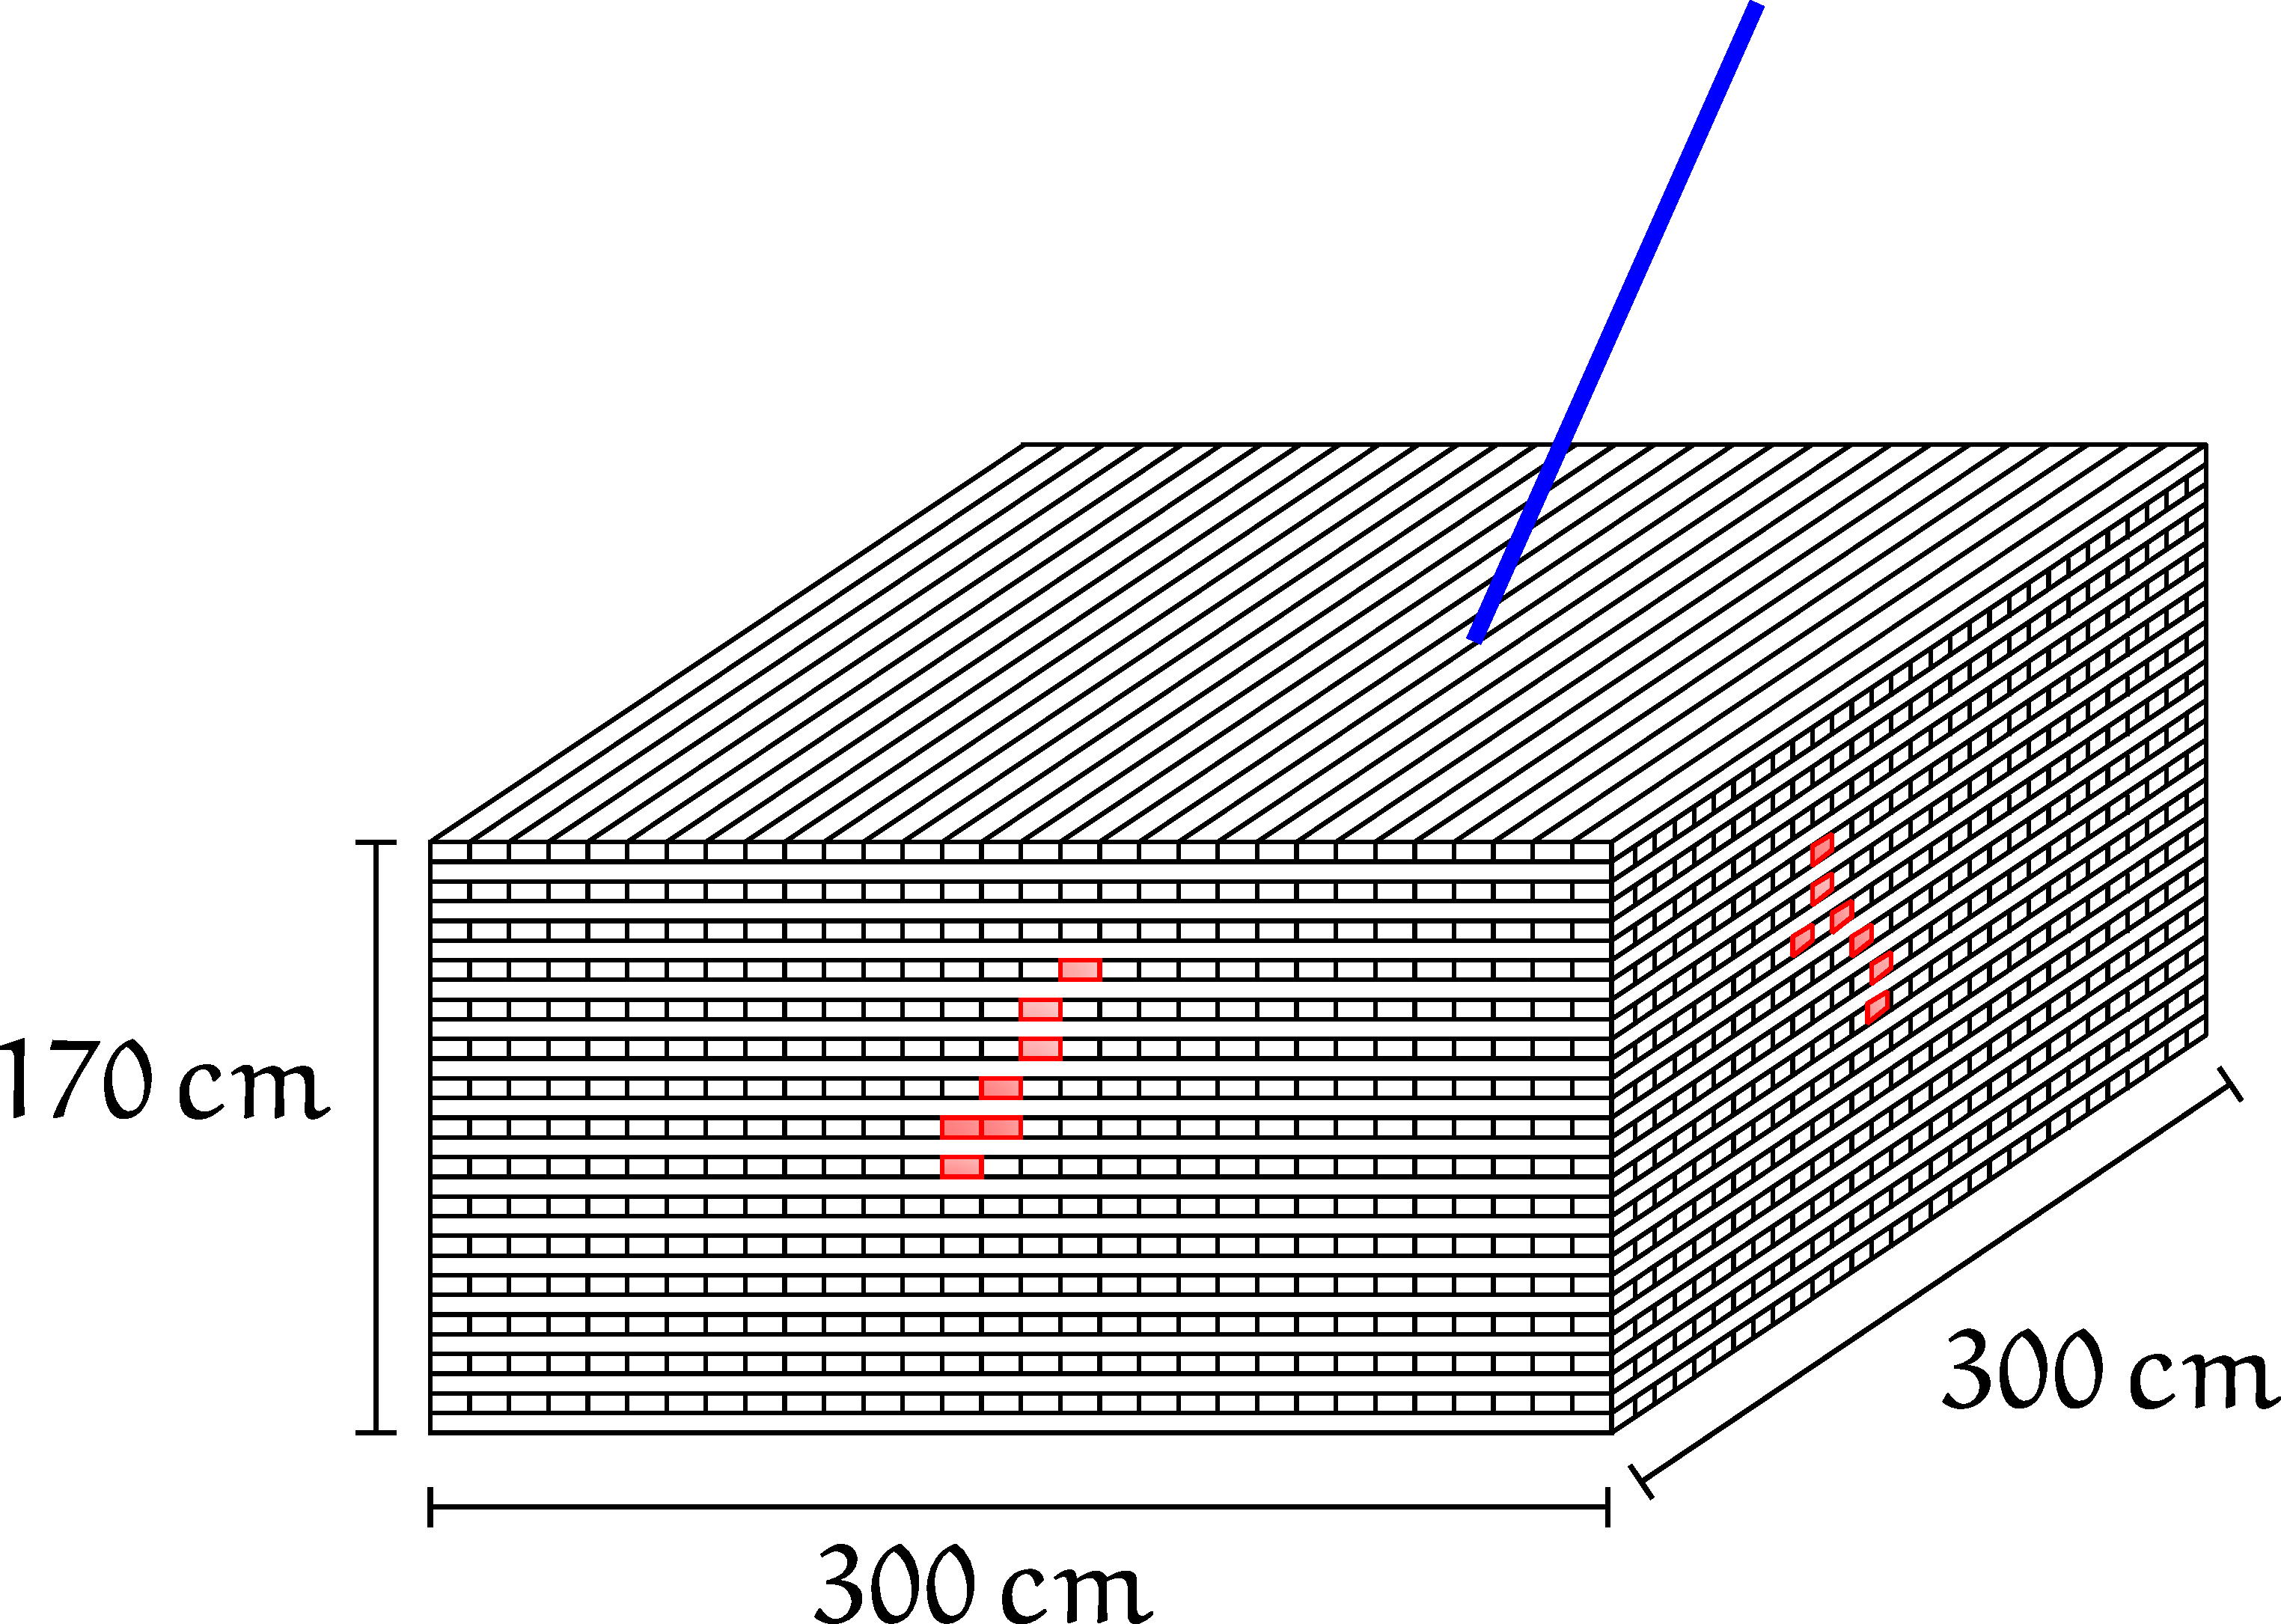
\includegraphics[width=0.7\textwidth]{scibar-diagram.pdf}
        \caption{Diagram esquemático del SciCRT. El detector se compone de \num{14848} barras centelladoras y fibras WLS. La lectura de las fibras se hace por medio MAPMTs en grupos de \num{64} canales.}
        \label{fig:scibar-detector}
\end{figure}

Por otro lado, dado que el SciCRT registra la energía depositada a lo largo la trayectoria de las partículas dentro del detector, podemos aplicar esquemas novedosos de identificación de partículas; lo cual a su vez mejora la sensibilidad a las partículas solares \cite{garcia20}. Este tipo de análisis \emph{offline} en conjunción con el uso de las barras de centelleo en modo anti-coincidencia mejora el rechazo a partículas de fondo (principalmente $\mu^{\pm}$ y rayos $\gamma$) incrementando la razón señal a ruido.

\section{Descripción del detector}

El SciCRT está compuesto de \num{14848} barras de centelleo, alineadas en planos horizontales $X-Y$, perpendiculares entre si. Los planos están constituidos de \num{116} barras en la dirección $X$ y \num{118} en la dirección $Y$. En total hay \num{128} capas de barras de centelleo apiladas verticalmente, agrupadas en estructuras de \num{16} capas llamadas \emph{Super block} (SB). Cada SB está sostenido firmemente por una estructura de acero, la cual mantiene la integridad mecánica de las barras. No obstante, la estructura introduce un hueco de aire entra cada capa de \SI{82}{\mm}; lo cual entre otras cosas afecta la respuesta angular del telescopio, por lo que es necesario incluir esta característica en las simulaciones del detector. El volumen total del barras en el detector es de \SI[product-units=power]{300x300x170}{\cubic\cm}.

Las barras de centelleo fueron fabricadas en el Fermilab y tienen características similares a las del experimento MINOS \cite{knitta04}. Están hechas de poliestireno, dopado con \SI{1}{\percent} PPO y \SI{0.03}{\percent} POPOP (ambos utilizados como \emph{cambiadores} de longitud de onda). Las dimensiones de las barras son \SI[product-units=power]{2.5x1.3x300}{\cubic\cm} y en el centro tienen un orificio cilíndrico de \SI{1.8}{\mm} donde se insertan fibras WLS (\emph{wavelength shifting}). Los centelladores tienen una cubierta de \ce{TiO2} (\SI{0.25}{\mm} de espesor) para aislarlos ópticamente entre si y mejorar la recolección de fotones. Un diagrama de las barras se observa en el panel izquierdo de la figura \ref{fig:scibar-optics}.

Las fibras WLS están acopladas por un lado a un tubo fotomultiplicador multi-ánodo (MAPMT) y por el otro extremo están pintadas de blanco para mejorar la eficiencia de recolección. Las fibras son del tipo Y11(200)MS desarrollado por la empresa \emph{Kuraray}. El fotomultiplicador es de \num{64} canales, modelo H8804, fabricado por \emph{Hamamatsu Photonics}.

El espectro de emisión de los plásticos centelladores se puede observar en el panel derecho de la figura \ref{fig:scibar-optics}, con una respuesta máxima a \SI{420}{\nano\metre}. Como se también se puede observar, el espectro de absorción de la fibra WLS está diseñado para cubrir de forma adecuada el espectro del plástico. La emisión de la fibra tiene un máximo a \SI{470}{\nano\metre}. La máxima eficiencia cuántica del MAPMT es de \num{0.25} a \SI{420}{\nano\metre}, pero disminuye a \num{0.15} al considerar la respuesta espectral del MAPMT.

\begin{figure}
        \centering
        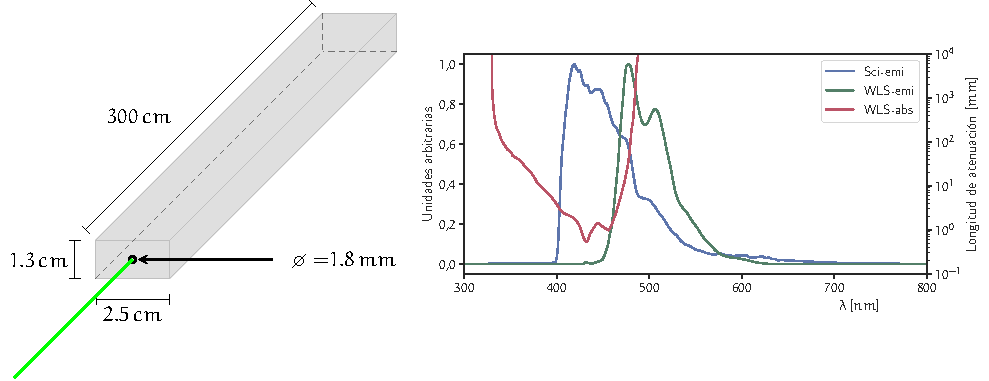
\includegraphics[width=\textwidth]{scibar.pdf}
        \caption{Diagrama esquemático de una barra centelladora con la fibra WLS instalada (panel izquierdo). Espectros de absorción y emisión de la fibra WLS y la barra de centelleo. Los datos de los espectros fueron obtenidos de \cite{kikawa14} y \cite{dietz16}.}
        \label{fig:scibar-optics}
\end{figure}

La electrónica para la adquisición de datos del telescopio fue desarrollada para el experimento K2K y está compuesta por circuitos de procesamiento analógico, de señal mixta y digitales; integrados a través de tecnología de alta escala \cite{myoshi04}. El procesamiento de la señales empieza con la conversión de la señal óptica en eléctrica por parte del MAPMT, para posteriormente ser amplificada, formada y multiplexada en la electrónica de \emph{Front End}. Este acondicionamiento se lleva a cabo en el dominio analógico y de señal mixta. Después de este proceso, las señales son multiplexadas y se transfieren a la electrónica de \emph{Back End} mediante un bus diferencial. En las unidades que integran la electrónica de BE las señales son convertidas a digital y transferidas finalmente al servidor de adquisición de datos mediante la interface VME. Para poder seleccionar los eventos a guardar, las unidades FE mandan una señal de \emph{hit} a las tarjetas de disparo (TRGB), las cuales son unidades de procesamiento digital programable que seleccionan los eventos con base en una condición de disparo.

Un diagrama esquemático de la electrónica instalada actualmente en el telescopio se muestra en la figura \ref{fig:scibar-electronics}. En el diagrama se muestra el flujo de señales, las cuales en el caso de los MAPMTs se procesan en paralelo por cada una de las FE y posteriormente son enviadas a las unidades BE para la conversión A/D. La TRGB recibe y envía señalizaciones al resto de la electrónica para indicar si se almacena el evento registrado. A partir de aquí podemos entender que la principal limitante  para el procesamiento de los eventos lo constituye el bus de comunicación al servidor. Para superar este obstaculo, la nueva versión de la electrónica utiliza el protocolo de comunicación Ethernet. Una discusión más profunda sobre este punto se encuentra en el capitulo \ref{chap:tres}, en donde además se listan la motivación científica y los requerimientos.

\begin{figure}
        \centering
        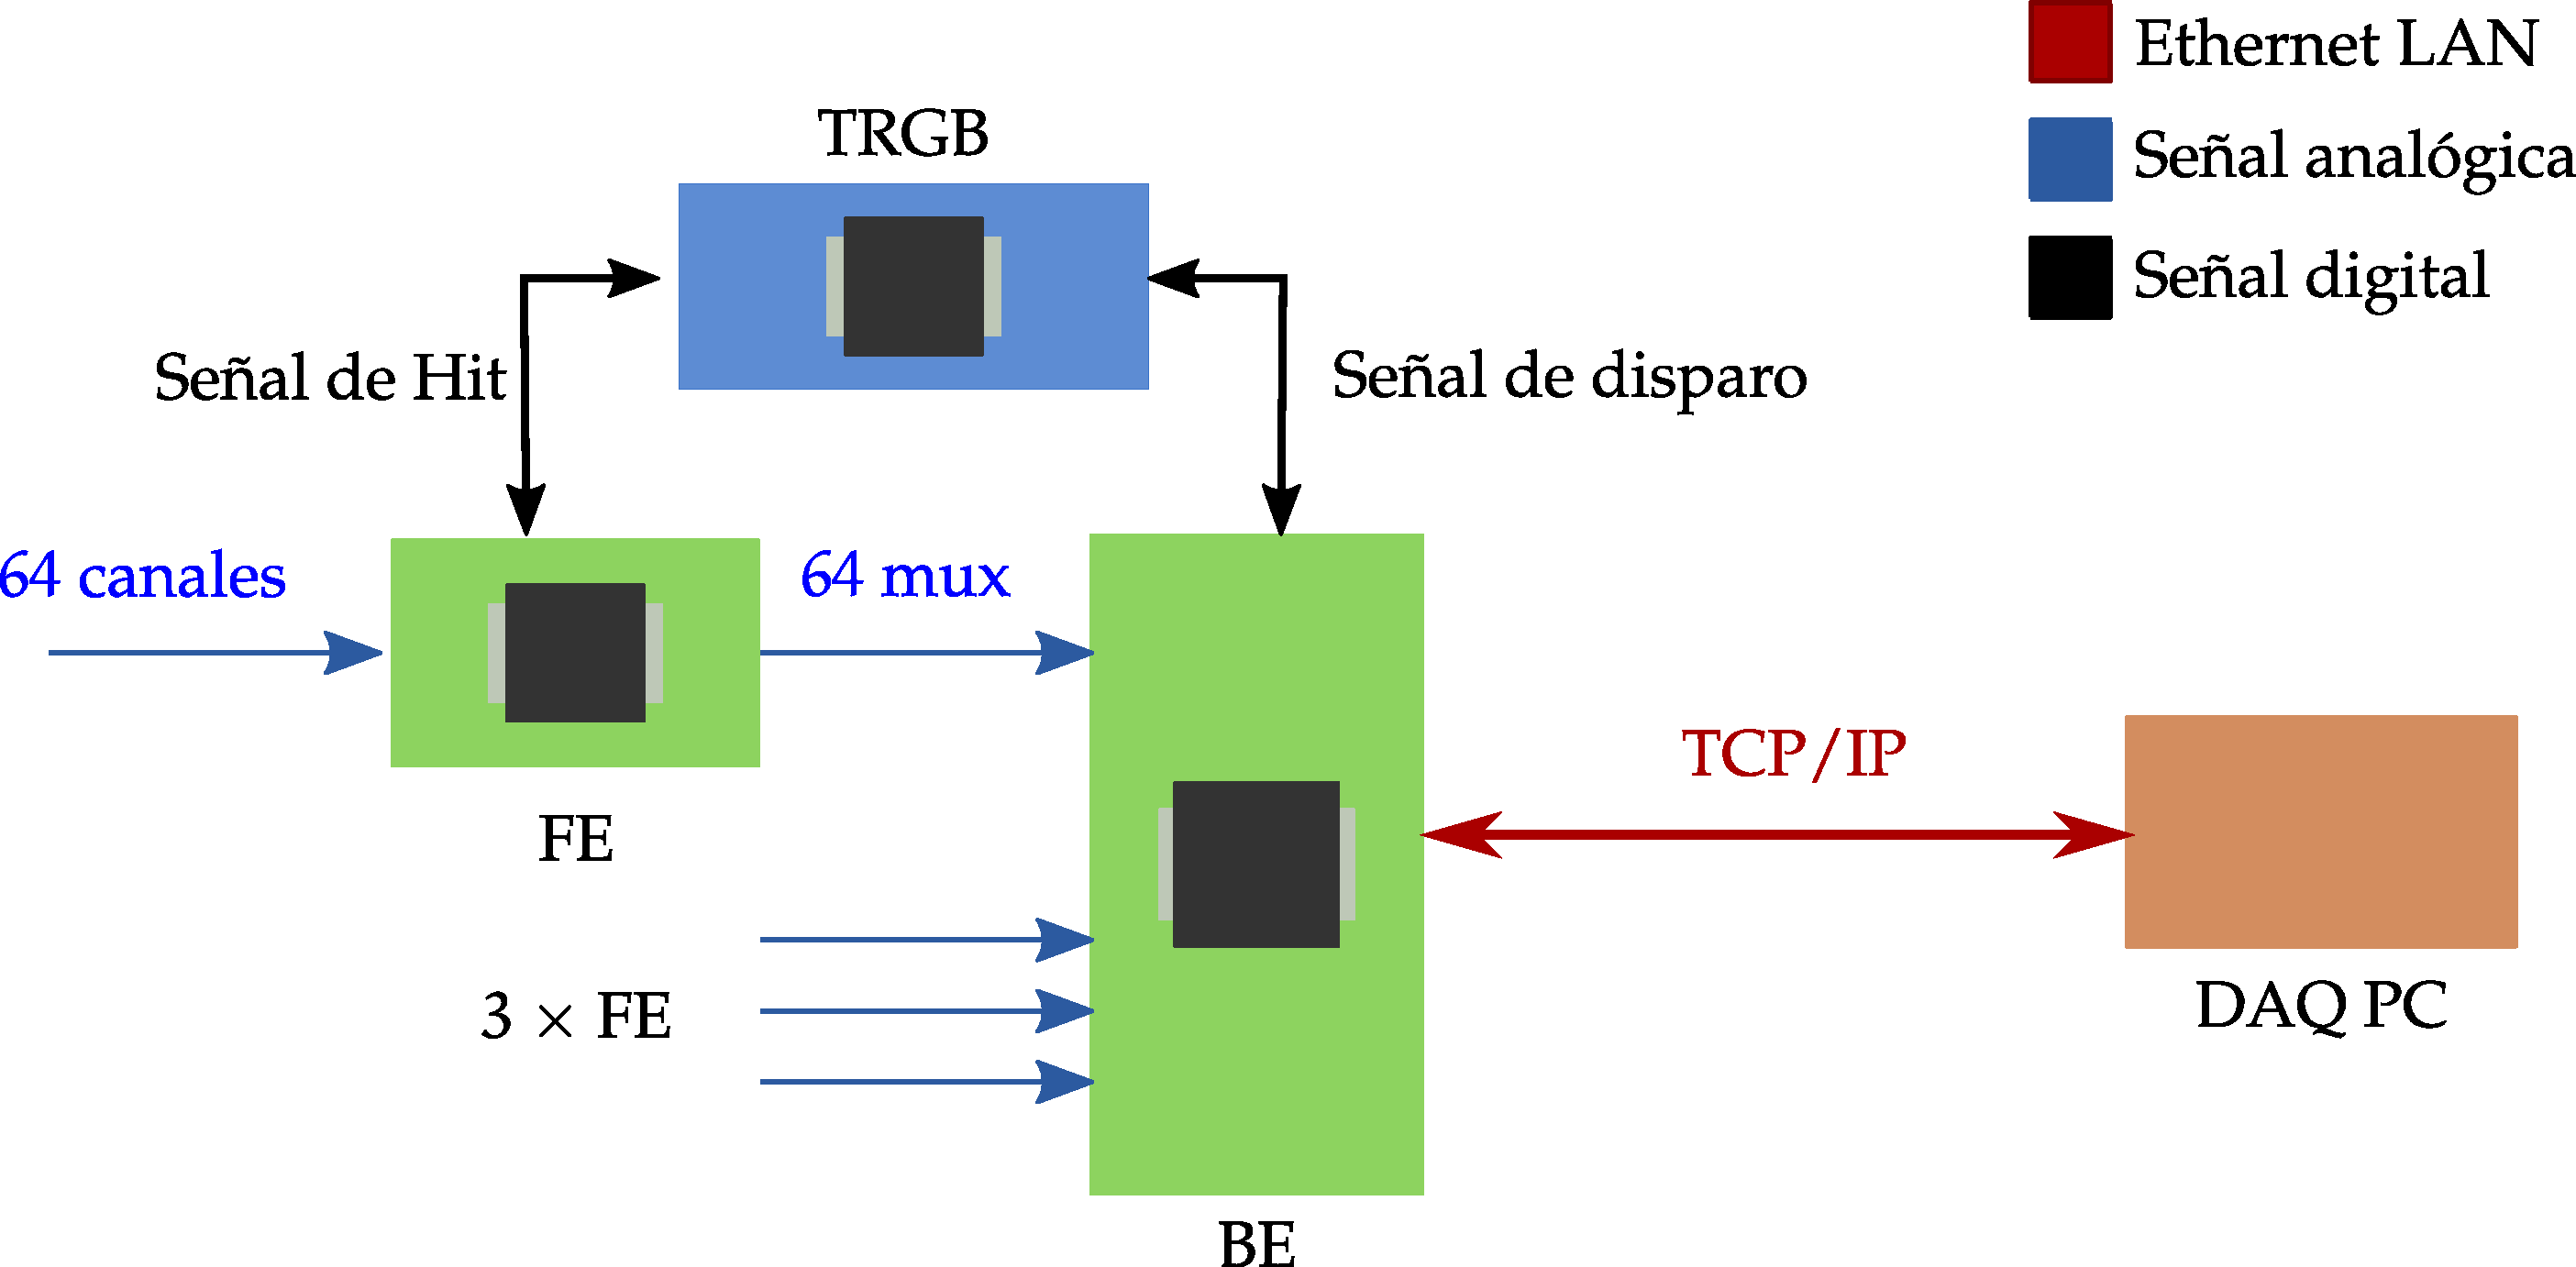
\includegraphics[width=\textwidth]{scicrt-electronics.pdf}
        \caption{Diagrama esquemático de la electrónica del SciCRT. La señal de los MAPMTs se procesan en paralelo en cada una de las FE y posteriormente son enviadas a las BE para la conversión A/D.}
        \label{fig:scibar-electronics}
\end{figure}

Bajo condiciones normales, el telescopio registra dos conjuntos de datos diferentes. Muones de alta energía (arriba de \SI{450}{\mega\electronvolt}) son detectados cuando producen coincidencia entre las capas superiores e inferiores del detector. El umbral para la detección de partículas en estas capas dedicadas es de \SI{0.3}{MIP} (\SI{\approx 0.5}{\mega\electronvolt}). El otro conjunto de datos del telescopio registra partículas neutras (aproximadamente \SI{70}{\percent} de los datos son de neutrones atmosféricos). El disparo para este tipo de eventos está definido cuando no hay ninguna señal en las capas de muones (anti-coincidencia) y además se registra una traza en uno de los SB con al menos \SI{14}{\mega\electronvolt} de energía depositada. Las ganancias de los MAPMT y umbrales para las capas de neutrones y muones se determinaron mediante simulaciones MC y se calibraron en Abril de \num{2014} \cite{ysasai14}.

\section{Caracterización del sistema óptico: barra de centlleo y fibra WLS}

Para lograr alcanzar los objetivos planteados el siguiente paso de mi investigación fue la caracterización de los elementos ópticos y optoelectrónicos que integran al SciCRT. Esto tuvo como objeto poder crear un modelo del proceso de generación de la señal de detección (simulación MC) y la posterior calibración de la electrónica usando dicho modelo.

Como ya mencioné anteriormente, las barras de centelleo del detector fueron fabricadas en Fermilab y han sido utilizados en diversos experimentos; por la misma razón sus propiedades ópticas y mecánicas han sido investigadas ampliamente. Como referencia me basé unicamente en los datos del fabricante \cite{beznosko}.

El fluor usado en los plásticos del SciCRT (POPOP y PPO) emite en el espectro visible desde aproximadamente \SI{400}{\nano\metre} hasta \SI{580}{\nano\metre}, con un máximo en \SI{420}{\nano\metre} \cite{kikawa14}. El espectro de emisión de la barra se puede observar en color azul en el panel derecho de la figura \ref{fig:scibar-optics}. Por otro lado, la figura \ref{fig:sim-optics} muestra el resultado de simular \num{1e6} muones interaccionando una barra centelladora descrita usando \emph{Geant4} \cite{geant403,geant406} (distribución en color azul). Las características del modelo de la barra descrito se resumen en la tabla \ref{table:optics}.

\begin{figure}
        \centering
        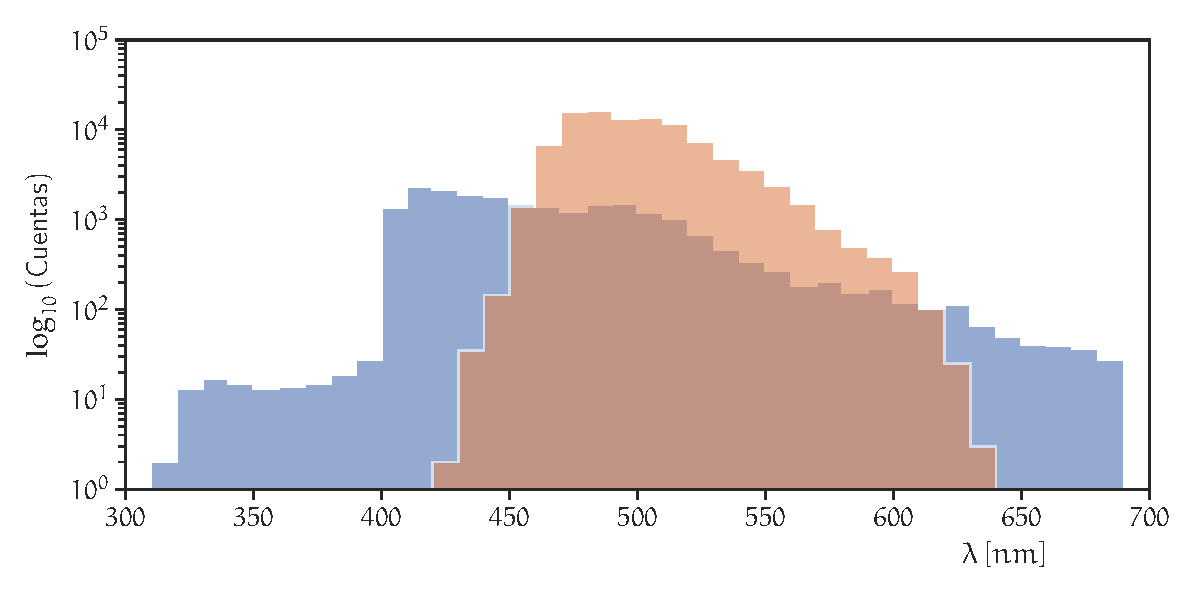
\includegraphics[width=\textwidth]{sim-optics-spect.pdf}
        \caption{Simulación MC del proceso de emisión-absorción de fotones entre la barra y la fibra WLS.}
        \label{fig:sim-optics}
\end{figure}

Al ser excitadas las moléculas de la barra, los fotones son emitidos de forma isotrópica en el volumen del plástico. Para mejorar la recolección por parte de la fibra WLS y para aislar ópticamente las barras entre si, cada centellador cuenta con un recubrimiento de \ce{TiO2}. El espesor del recubrimiento impone una cota minima en la energía del primario que puede entrar en la barra y producir una señal detectable. De acuerdo con \cite{gros18}, resultados de una simulación MC sugieren que con un espesor similar al de las barras del SciCRT; el flujo de protones, electrones y fotones con $E_{k}<\SI{10}{\mega\electronvolt}$ es atenuado considerablemente. En el caso de nuestro detector este efecto es despreciable ya que, a partir de nuestra  simulación sabemos que el umbral de detección de primarios (para las especies antes mencionadas) se encuentra cercano a \SI{100}{\mega\electronvolt}.

En nuestra simulación de la barra un aspecto de vital importancia para la generación de las señales ópticas es el acoplamiento óptico que existe entre la superficie de la barra y el revestimiento. Tomando en consideración \cite{dietz16,gros18}, fijé la reflectividad del recubrimiento en \SI{90}{\percent} en el rango de \SI{300}{\nano\metre} a \SI{800}{\nano\metre}, considerando además una componente difusa y especular. Dicho de otra forma, esta caracterización garantiza que la simulación trata la reflexión de los fotones en el recubrimiento principalmente de manera geométrica, ensanchando el espectro de los fotones de acuerdo a un cierto parámetro de rugosidad. Esto permite simular las imperfecciones en ambas superficies.

Una fracción de los fotones que llegan a entrar en la fibra WLS son absorbidos y reemitidos a una mayor longitud de onda que la inicial\footnote{Por efecto de la conservación de la energía el fotón reemitido nunca puede tener una longitud menor a la longitud inicial.}. La emisión de los fotones por la fibra tiene las características de un decaimiento exponencial con $\lambda_{WLS}=\SI{12.0}{\nano\second}$ y es isotrópica. Debido a que la fibra tiene dos recubrimientos (metacrilato y metacrilato fluorado), para que se lleve a cabo la reflexión total interna se requiere que los fotones sean emitidos con ángulos menores a \SI{26.9}{\degree} con respecto al eje de la fibra \cite{kikawa14}.

\begin{table}
\caption{Características ópticas y mecánicas.}
\label{table:optics}

\begin{tabular}{lr}

\multicolumn{2}{c}{}\\
\cmidrule(r){1-2}
\addlinespace[5pt]
\textbf{(a) Barra centelladora}\\
\addlinespace[5pt]
\cmidrule(r){1-2}
Material base & poliestireno\\
Fluor & PPO y POPOP\\
Densidad (\si{\gram\per\cubic\cm}) & \num{1.08}\\
Pico de emisión (\si{\nm}) & \num{420}\\
Constante de decaimiento (\si{\ns}) & \num{3.6}\\
Constante de Birks (\si{\cm\per\mega\electronvolt}) & \num{0.0208}\\
Producción de luz (\si{fotones\per\mega\electronvolt}) & \num{8000}\\
Dimensiones (\si{\cubic\cm}) & \num[product-units=power]{2.5x1.3x300}\\
\addlinespace[10pt]
\textbf{(b) Fibra WLS Y11(200)}\\
\addlinespace[5pt]
\cmidrule(r){1-2}
Densidad (\si{\gram\per\cubic\cm}) & \num{1.05}\\
Pico de emisión (\si{\nm}) & \num{470}\\
Longitud de absorción & ver figura \ref{fig:scibar-optics}\\
Índice de refracción (núcleo) & \num{1.60}\\
Índice de refracción (revestimiento 1) & \num{1.49}\\
Índice de refracción (revestimiento 2) & \num{1.42}\\
Tiempo de decaimiento (\si{\ns}) & \num{12.0}\\
Reflectancia de la pintura & 0.54\\
\addlinespace[10pt]
\textbf{(c) MAPMT H8804}\\
\addlinespace[5pt]
\cmidrule(r){1-2}
Longitud de onda de respuesta máxima(\si{\nm}) & \num{420}\\
QE máxima (\si{\percent})  & \num{25}\\
Ganancia a \SI{-950}{\volt} & \num{5.9e6}\\
Tiempo de levantamiento (\si{\ns}) & \num{1.0}\\
\addlinespace[5pt]
\bottomrule

\end{tabular}
\end{table}

Los parámetros usados en la simulación de la fibra en Geant4 se muestran en la tabla \ref{table:optics}. Es importante hacer notar que todos los parámetros ópticos utilizados fueron definidos en el rango de \SI{300}{\nano\metre} a \SI{800}{\nano\metre}, lo cual requirió en algunos casos extrapolar cuidadosamente los datos proporcionados por el fabricante. Relacionado a este punto, ese necesario evitar introducir discontinuidades en los espectros definidos, ya que dicha situación conlleva a la creación de acoplamientos ópticos artificiales y por lo tanto a la atenuación de la señal óptica. En la figura \ref{fig:sim-optics}, la distribución en color naranja muestra los fotones reemitidos en la simulación, los cuales constituyen una prueba de la consistencia de la simulación.

Dentro de los parámetros de la simulación, la longitud de atenuación óptica de la fibra WLS requirió una calibración especial. La figura \ref{fig:atlength} muestra los resultados de este procedimiento. Como primer paso, la línea naranja es el resultado de la simulación previo a la calibración. La simulación consistió en arrojar fotones usando el espectro de emisión de la barra, a diferentes posiciones fijas dentro de la fibra y de manera isótropica. En la simulación usé como parámetro de entrada la longitud de atenuación propuesta por el fabricante: $>\SI{3500}{\milli\metre}$, la cual se define en Geant4 como una propiedad del material (en este caso del núcleo de la fibra). Para cada posición la simulación registra el número de fotones que llegaron al extremo de la barra donde se encuentra el fotosensor. Luego entonces, los resultados en la figura \ref{fig:atlength} son el número de fotones (normalizado) $L(x)$ que alcanzan el MAPMT en función de la distancia al mismo.

Los resultados de la simulación se pueden ajustar con la ecuación \ref{equ:fiber-att}, la cual representa la relación entre la distancia al fotomultiplicador y $L(x)$:

\begin{equation}
\label{equ:fiber-att}
L(x)=k\left(\exp\left(-\frac{x}{\lambda}\right) +R\exp\left(-\frac{2.0x_{tot}-x}{\lambda}\right)\right)
\end{equation}

de donde $k$ es la ganancia del sistema óptico, $\lambda$ es la longitud de atenuación, $R$ es la reflectancia de al final de la fibra WLS y $x_{tot}$ es la longitud total de la fibra (aproximadamente \SI{330}{\cm}, incluyendo la distancia del borde de la barra al fotomultiplicador). De manera general, el primer término de la ecuación representa la fracción de la luz que llega al MAPMT directamente, mientras que el segundo término representa la fracción reflejada.

\begin{figure}
        \centering
        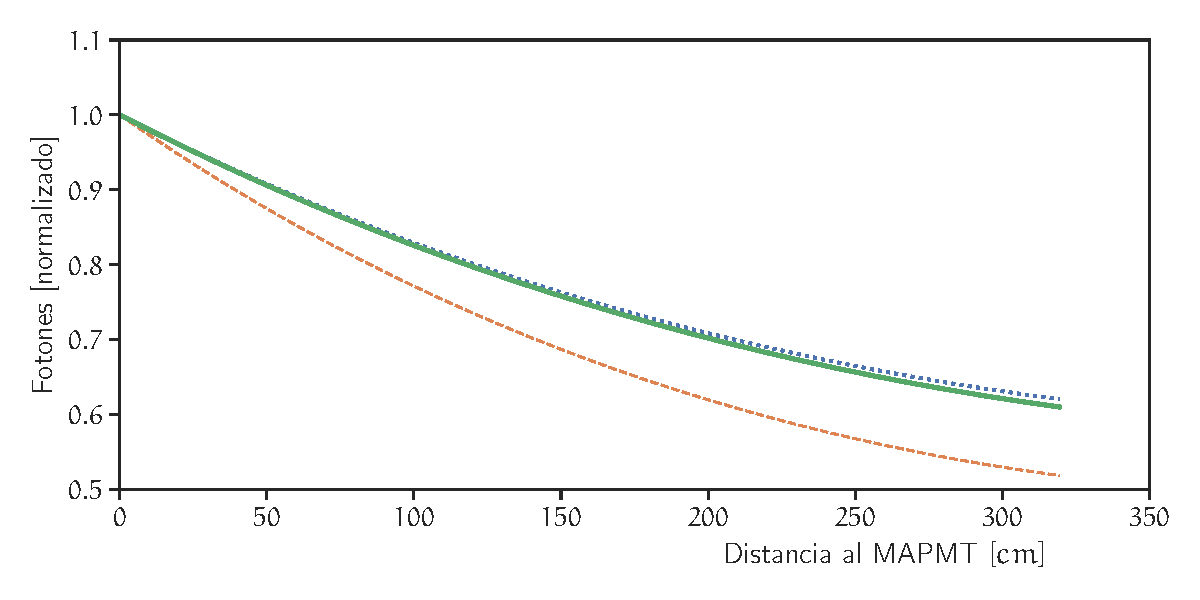
\includegraphics[width=\textwidth]{data_atlength.pdf}
        \caption{Atenuación de fotones en la fibra WLS. La línea azul son datos del experimento. La línea naranja representa el resultado de la simulación MC usando la atenuación reportada por el fabricante. La línea verde es el ajuste de la simulación a partir del experimento.}
        \label{fig:atlength}
\end{figure}

El siguiente paso fue la obtención de la longitud de atenuación usando los datos del telescopio. Para determinar este parámetro usé \num{\sim 4e6} eventos de muones, los cuales fueron registrados usando como disparo la coincidencia de las capas superiores e inferiores del detector (\emph{$4$-fold}). Utilicé muones para esta prueba debido a que son partículas de ionización mínima (MIP) y su deposición de energía en una barra es prácticamente constante (aproximadamente \SI{1.8}{\mega\electronvolt}).

A partir de los datos registrados, construí distribuciones de la energía depositada en cada barra de uno de los lados del detector; mientras la traza en la otra cara del detector sirve para medir la distancia entre el punto de cruce de la partícula y el MAPMT. Las distribuciones de cada barra se clasifican en $14$ grupos diferentes (hay \num{14} MAPMTs en una de las caras del SciCRT), lo cual hace posible medir el efecto de atenuación en la fibra midiendo la posición del pico de la distribución de energía depositada en cada barra. Utilizando esta clasificación es posible medir la distancia del punto de cruce con un incertidumbre de \SI{\pm 10}{\cm}. Una restricción extra que establecí en el análisis fue la de analizar solo eventos producidos por partículas que cruzan de forma vertical, lo cual tiene por objetivo evitar eventos con una larga deposición de energía. La figura \ref{fig:muon-selection} muestra de forma resumida el procedimiento de selección de eventos y clasificación descrito. La barra en color azul es el canal que estamos analizando (panel izquierdo), mientras que las barras rojas en el otro lado del detector sirven para medir la distancia al MAPMT y seleccionar eventos verticales (panel derecho).

Por otro lado la figura \ref{fig:adc-distance} muestra las distribuciones de ADC de muones cruzando a dos distancias diferentes del MAPMT. La distribución en azul claro corresponde a una distancia de \SI{280}{\cm}, mientras que la distribución en azul oscuro la obtuve a \SI{40}{\cm}. Usando un voltaje de alimentación \SI{-900}{\volt} para cada MAPMT, cerca del \SI{50}{\percent} de las barras (de un total de \num{896}) tiene estadística suficiente para realizar el análisis, lo cual quiere decir que las distribuciones obtenidas no son afectadas por la saturación del MAPMT o falta de ganancia.

\begin{figure}
        \centering
        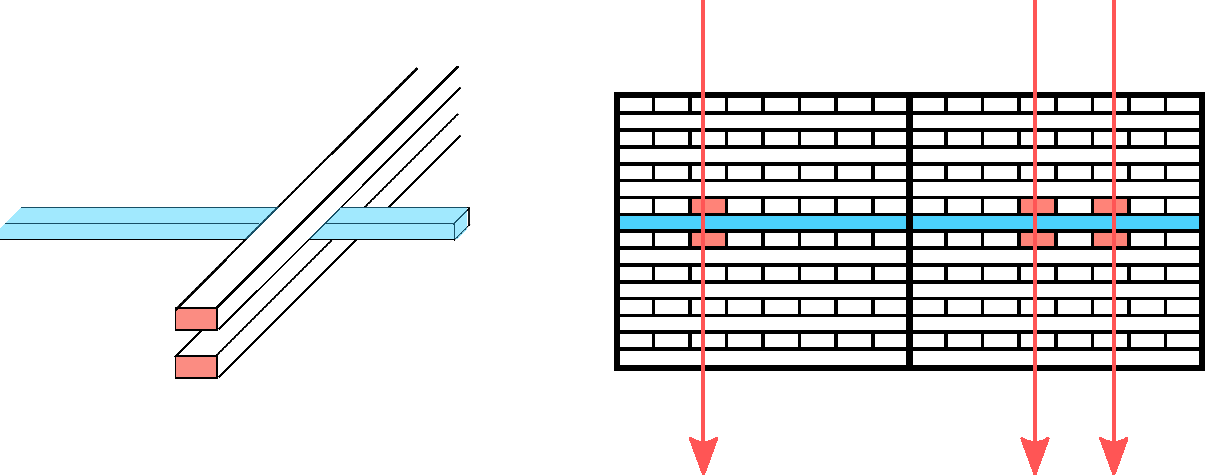
\includegraphics[width=\textwidth]{muon-attenuation.pdf}
        \caption{Diagrama esquemático de la selección de eventos de muones en los datos del SciCRT.}
        \label{fig:muon-selection}
\end{figure}

\begin{figure}
        \centering
        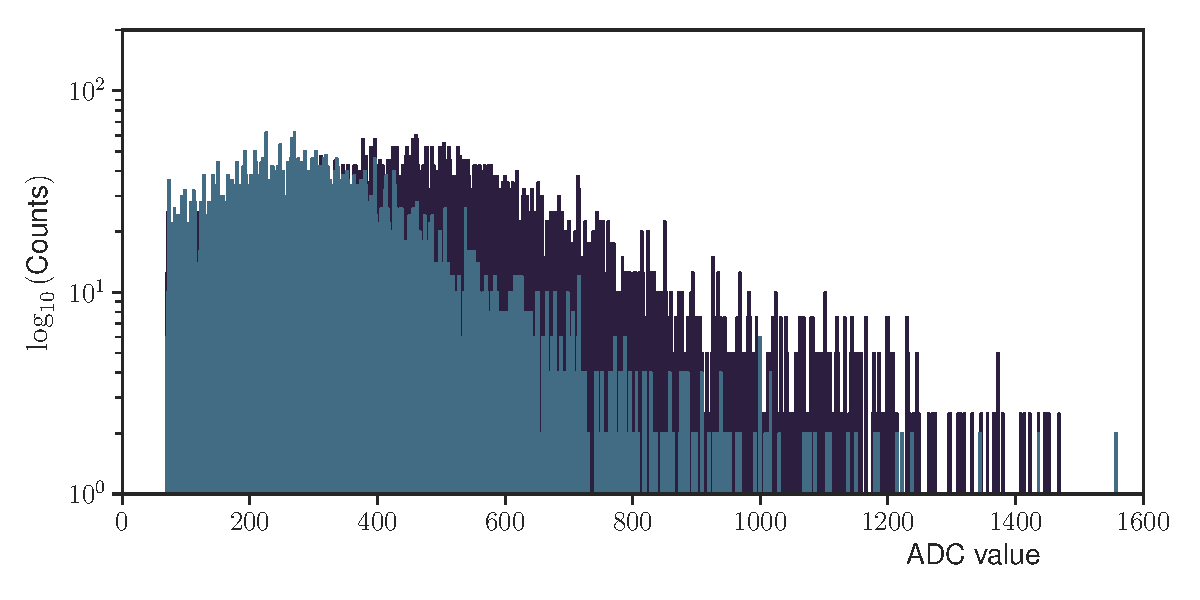
\includegraphics[width=\textwidth]{adc_attenuation.pdf}
        \caption{Distribuciones de ADC de muones que cruzan una barra de centelleo a diferentes distancias del fotomultiplicador.}
        \label{fig:adc-distance}
\end{figure}

Ya que los muones registrados en el análisis están el rango de energía de \num{0.5} a \SI{30}{\giga\electronvolt} y son considerados MIPs, las distribuciones de intensidad luminosa registrada por los MAPMTs pueden ser ajustadas utilizando distribuciones de Landau. A partir del valor máximo estimado en cada ajuste (MPV) procedí a calcular el promedio ponderado para cada distancia. Posteriormente, ajusté la ecuación \ref{equ:fiber-att} y como resultado obtuve la gráfica azul mostrada en el figura \ref{fig:atlength}. Los parámetros obtenidos a partir del ajuste son: $\lambda=\SI{408(4)}{\cm}$ y $R=\num{0.541(30)}$, lo cual es consistente con un estudio previo \cite{itow13}.

No obstante, es evidente de la figura que el resultado experimental difiere del obtenido en la simulación, lo cual indica que es necesario ajustar los parámetros del código. La discrepancia entre ambos experimentos proviene de varios factores. El primero es que la longitud de atenuación provista por el fabricante es en realidad un \emph{longitud de atenuación de señal}, es decir, proviene de una medición realizada por el fabricante en donde interviene la geometría del experimento donde se midió y el acoplamiento óptico entre los diferentes elementos. En comparación el valor asignado en la simulación, la longitud de atenuación es una propiedad del material.

Con objeto de resolver esta discrepancia en \cite{dietz16} se propone utilizar el espectro de pérdidas de señal $\mu_{WLS}$, el cual se muestra en la figura \ref{fig:sim-optics} y describe de mejor forma la atenuación en la fibra. Este espectro es provisto por el fabricante, sin embargo requiere la corrección mediante un factor de cuadrático, de la siguiente forma:

\begin{equation}
\label{equ:quadcorr}
\mu_{corr}=a_{0}\cdot\mu_{WLS}+a{1}\cdot\mu^{2}_{WLS}
\end{equation}

en donde $\mu_{corr}$ es el espectro corregido y $\mu_{WLS}$ es el especificado por el fabricante. De esta forma podemos usar las constantes $a_{0}$ y $a_{1}$ para calibrar los resultados de la simulación con el experimento. Finalmente, la linea verde en la figura \ref{fig:atlength} muestra el resultado de la corrección de la simulación, con parámetros de ajuste: $\lambda=\SI{405(3)}{\cm}$ y $R=\num{0.498(20)}$. A partir de esto podemos concluir que la atenuación óptica en la simulación concuerda con el experimento.

\section{Formación de la señal de detección y respuesta del fotomultiplicador}

La interacción de una partícula en el centellador produce un enorme número de fotones, de los cuales una pequeña fracción es capturada en la fibra WLS y puede propagarse a uno de los pixeles del MAPMT. En consecuencia, la señal eléctrica que debe procesar la instrumentación, es una señal de corriente compuesta por la suma de las contribuciones individuales de cada fotón que fue detectado por el sensor óptico. Así el modelo de señal eléctrica se puede definir a través de la siguiente ecuación:

\begin{equation}
\label{equ:current-pulse}
i_{pmt}\left(x,t\right)=\sum_{i=1}^{N_{phe}}i\left(t-t_{i}\right)
\end{equation}

de donde $i_{pmt}$ es la corriente a la salida del MAPMT en función del tiempo y posición en la que atravesó la partícula la barra; $N_{phe}$ es el número total de fotoelectrones a la salida del MAPMT y $t_{i}$ la distribución de los tiempos de arribo. Es importante mencionar que $N_{phe}$ a su vez depende de la distancia, la ganancia del MAPMT, eficiencia cuántica y energía depositada por la partícula en la barra. A continuación dedicaré mi esfuerzo en presentar las características temporales de la señal de detección

Los fotones que la fibra logra transportar hacia alguno de los fotocátodos del sensor tienen una distribución de tiempo definida principalmente por dos variables aleatorias \cite{sanchez10}. La primera de éstas es, a su vez, la suma de dos variables aleatorias; la desexecitación de la fibra WLS y la emisión por parte del material centellador debido al paso de radiación ionizante. Ya que ambos procesos son independientes entre si y pueden ser descritos mediante variables aleatorias exponenciales, la siguiente ecuación describe la distribución de tiempos $P_{D}$ resultante:

\begin{equation}
\label{equ:exponential-decay}
P_{D}(t)=\frac{e^{-t/t_{p}}-e^{-t/t_{f}}}{t_{p}-t_{f}}
\end{equation}

de donde $t_{p}$ y $t_{f}$ son las constantes de decaimiento de la barra y fibra WLS, respectivamente. Valores característicos para estos parámetros se pueden ver en la tabla \ref{table:optics}, los cuales fueron  determinados en experimentos previos \cite{gros18,mineev11}. Una observación importante al respecto es, dado que la fibra WLS tiene una constante de decaimiento mayor a la de la barra (\SI{12}{\nano\second}); es la primera la que domina el proceso.

La segunda variable aleatoria que afecta las distribuciones de tiempo de los fotones es la relacionada con la propagación en la fibra. Considerando solo los fotones que tienen una propagación meridional, el tiempo que tardan en recorrer la fibra se puede estimar de la siguiente forma:

\begin{equation}
\label{equ:meridional}
t_{prop}=\frac{x}{\cos(\alpha)}\frac{n_{core}}{c}
\end{equation}

donde $\alpha$ representa el ángulo con respecto al eje de la fibra y es una variable aleatoria uniforme; $c/n_{core}$ es la velocidad de los fotones en el medio y $x/\cos(\alpha)$ la distancia recorrida total por el fotón hasta un pixel del MAPMT. No obstante, el tiempo real de propagación de un fotón en la fibra se ve afectado directamente por la pintura al final de la fibra y las reflexiones ocurridas en el recubrimiento del plástico. Luego entonces, si consideramos el \emph{paquete} de fotones que se propaga por la fibra después de la interacción, el efecto general del proceso de transporte es la atenuación y ensanchamiento del pulso luminoso. Ambos efectos son de gran importancia en el contexto del desarrollo de electrónica de alta velocidad.

La distribución temporal de los fotones que llegan al MAPMT es finalmente afectada por la respuesta del mismo. A continuación describiré brevemente el principio de funcionamiento del sensor y sus propiedades.

El fotomultiplicador convierte la señal óptica débil en una señal eléctrica, con alta ganancia, bajo ruido y baja distorsión. Cuando los fotones llegan al fotocátodo, los electrones que se encuentran en la banda de valencia absorben la energía de los primeros ($h\nu$). Si la energía adquirida por los electrones es mayor que la función de trabajo del material, éstos son emitidos como fotoelectrones. Dependiendo de la eficiencia del material fotosensible y la energía de los fotones incidentes, una fracción de éstos provocará la emisión de electrones.

Los fotoelectrones emitidos son acelerados por el campo eléctrico de los dínodo. En el dínodo la multiplicación de electrones se lleva a cabo a través de la emisión secundaria de electrones. Para alcanzar ganancias superiores a \num{e4}, un fotomultiplicador necesita varias etapas de emisión. Para el caso los MAPMTs en el SciCRT la ganancia puede alcanzar \num{e7} utilizando \num{12} dínodos.

Los fotomultiplicadores son detectores con respuesta extremadamente rápida. Sus características están principalmente determinadas por el \emph{tiempo de tránsito} que requieren los fotoelectrones emitidos por el fotocátodo en a travesar la estructura multiplicadora y llegar al ánodo \cite{hama07}. A pesar de esto, a causa de la naturaleza aleatoria del proceso de emisión secundaria, el tiempo de tránsito no es constante, sino tiene una distribución. Esto implica que la respuesta del sensor a un pulso muy corto de luz siempre tendrá un ensanchamiento finito y variable \cite{syed07}. Al ancho total a altura media (FWHM) de la función de densidad de los tiempos de tránsito se le conoce como: \emph{spread in transit time}.

La respuesta espectral de los sensores utilizados en el SciCRT es proporcionada por el fabricante y está resumida en la tabla \ref{table:optics}. De aquí es importante notar que aunque la eficiencia cuántica máxima es cercana al \SI{30}{\percent}, en realidad cuando consideramos en su totalidad la respuesta espectral del sensor la eficiencia está más próxima al \SI{15}{\percent}.

Por otro lado, sobre la respuesta temporal del MAPMT no existe documentación abierta al respecto. Para lograr caracterizar este elemento buscaremos obtener el \emph{single photo-electron response} del fotomultiplicador; el cual se define cómo el estado en el que el sensor responde en promedio con un solo fotoelectrón por pulso luminoso incidente. Para obtener esta respuesta desarrollé un experimento colocando al MAPMT en una caja negra e iluminé la superficie fotosensible con un pulso de muy corta duración. Para evitar la saturación del sensor, coloqué el sensor a una distancia de \SI{50}{\cm}, además de utilizar un difusor. En este caso el difusor fue un cono de plástico pitado de blanco, el cual produce un haz luminoso homogéneo.

La fuente luminosa la cree utilizando un diodo emisor de luz (LED), un circuito digital para generar los pulsos de alimentación (del orden de \SI{100}{\nano\second}) y un circuito diferenciador RC.

Para realizar correctamente la prueba, previo a la iluminación del fotocátodo, medí los niveles de ruido de la cámara oscura para garantizar un nivel adecuado de cuentas por corriente oscura. El nivel de ruido para pulsos de \SI{-10}{\milli\volt} de amplitud es de \SI{0.5}{cuentas\per\second}.

Los resultados del experimento usando la fuente luminosa se muestran en la figura \ref{fig:sphe}. La línea negra representa la respuesta promedio obtenida de probar con \num{7} MAPMTs, mientras que el área sombreada representa la variación de $\pm\sigma$. El LED que utilicé tiene un máximo en su respuesta de \SI{505}{\nano\metre}. Ya que la respuesta temporal del fotomultiplicador tiene un ancho de banda muy grande, para la digitalización de los pulsos utilicé un osciloscopio de alta resolución  (ancho de banda de \SI{2}{\giga\hertz} y frecuencia de muestreo de \SI{10}{\giga muestras\per\second}), que fue facilitado por el Laboratorio de detectores del Instituto de Ciencias Nucleares.

\begin{figure}
        \centering
        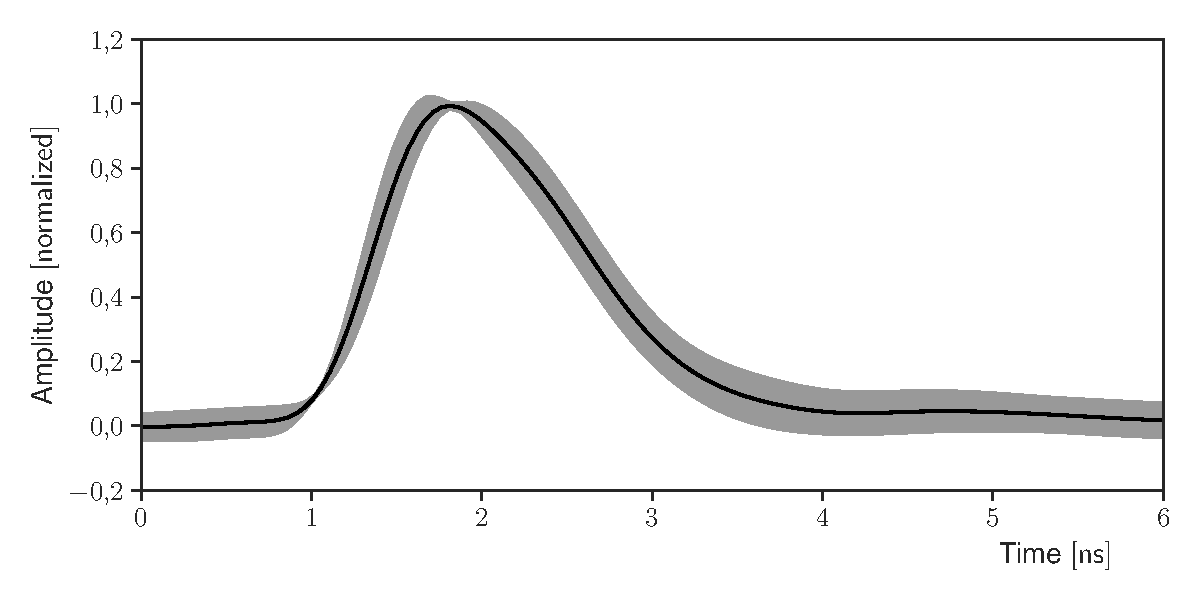
\includegraphics[width=\textwidth]{sphe-signal.pdf}
        \caption{Respuesta SPE promedio en función del tiempo (linea negra). El área sombreada muestra las fluctuaciones de $\pm\sigma$.}
        \label{fig:sphe}
\end{figure}

Para lograr el estado SPE ajusté la intensidad de luz de tal manera que tuviera un \SI{10}{\percent} de eventos detectados, lo cual basados en estadística de Poisson garantiza un \SI{\sim 0.5}{\percent} de eventos contienen $2$ o más fotoelectrones \cite{barnhill08}.

De acuerdo con \cite{sanchez10}, la respuesta SPE puede ser modelada como la respuesta en el tiempo de un circuito $CR-(RC)^{\alpha}$ como sigue:

\begin{equation}
\label{equ:sphe}
v(t)=\frac{QR}{\tau\Gamma(1+\alpha)}\left(\frac{t}{\tau}\right)^{\alpha}\mathrm{e}^{-t/\tau}
\end{equation}

en donde $Q$ es la carga integrada del pulso (o carga característica), $R$ es la resistencia de carga y
$\tau$ y $\alpha$ son parámetros libres del modelo. $\Gamma(1+\alpha)$ es la función gamma la cual se usa como constante de normalización.

Para poder ajustar este modelo a los datos primero obtuve las distribuciones de $Q$ para diferentes voltajes de operación: \SI{-850}{\volt},\SI{-900}{\volt} y \SI{-950}{\volt}, lo cual se muestra en la figura \ref{fig:mapmt_charge}. Estas distribuciones se pueden aproximar utilizando una distribución Gaussiana. Con un voltaje de alimentación de \SI{-950}{\volt} la carga media medida es de \SI{0.938(3)}{\pico\coulomb}. Siguiendo un procedimiento similar para las distribuciones de $\tau$ (las cuales se ajustan más a una distribución de Landau) obtuve un valor de $\alpha=2.0$ para nuestro MAPMT.

\begin{figure}
        \centering
        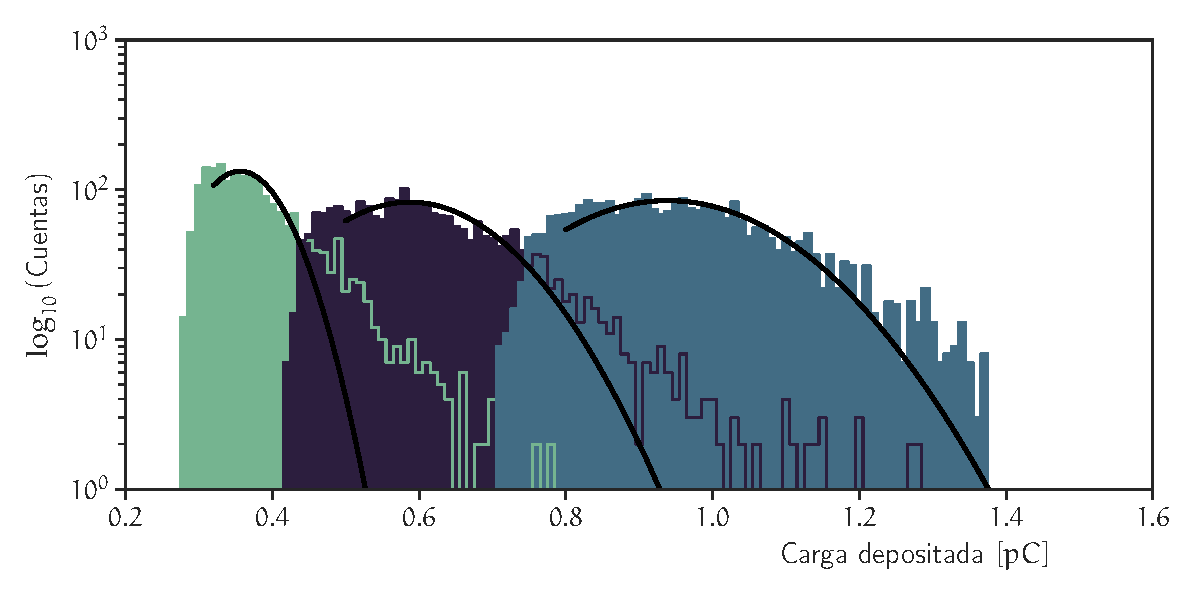
\includegraphics[width=\textwidth]{mapmt_charge.pdf}
        \caption{Distribuciones de carga de SPE para tres diferentes voltajes de operación. De izquierda a derecha los voltajes utilizados son: \SI{-850}{\volt},\SI{-900}{\volt} y \SI{-950}{\volt}.}
        \label{fig:mapmt_charge}
\end{figure}

De esta manera, la caracterización de los elementos optoelectrónicos que intervienen en la formación de la señal me permitió crear un modelo de la misma, el cual incluye propiedades medidas experimentalmente y procesos físicos relevantes; y nos permitirá un estudio detallado para el desarrollo de nuestro instrumento. Ésto, sin embargo, será el objetivo del siguiente capítulo. La siguiente sección está dedicada a la validación experimental de la simulación Monte Carlo.

\section{Validación experimental de la simulación}

El experimento que desarrollé para validar la simulación consiste en detectar $\mu^{\pm}$ usando la coincidencia de \num{4} barras centelladoras ubicadas en las capas superiores e inferiores del detector, como muestra en la figura \ref{fig:muons-experiment-0}. En la figura, las barras con las que se realiza la coincidencia están etiquetadas de $p_{0}$ a $p_{3}$. Considerando las dimensiones de las barras (\SI{2.5}{\cm} de ancho), el área total de detección es de \SI{6.25}{\cm\squared}. Si además tomamos en cuenta que existe una distancia de \SI{200}{\cm} entre las barras superiores e inferiores, el ángulo máximo con respecto al cenit con que los $\mu^{\pm}$ pueden generar coincidencia es de \SI{0.36}{\degree}.

Los \SI{200}{\cm} de material centellador (aproximadamente \num{128} barras) también imponen un límite inferior a la energía cinética de los muones detectados. Una primera estimación se puede hacer utilizando la ecuación de Bethe-Bloch:

\begin{align}
\label{equ:bethe}
\frac{\mathrm{d}E}{\mathrm{d}x} &=-2a\left[\frac{1}{2}\ln\left(\frac{2m_{e}\beta^{2}\gamma^{2}w_{max}}{\bar{I}^{2}}\right)-\beta^{2}-\frac{\delta}{2}\right] \\
a &=2\pi N_{e}r_{e}^{2}m_{e}z_{\beta}  \nonumber \\
w_{max} &=\frac{2m_{e}\beta^{2}\gamma^{2}}{1+2m_{r}\gamma+m_{r}^{2}} \nonumber
\end{align}

con $r_{e}=\SI{2.818e-13}{\cm}$ el radio clásico del electrón; $\gamma$ el factor de Lorentz; $\beta=v/c$, $m_{e}=\SI{0.511}{\mega\electronvolt\per c^{2}}$ la masa en reposo del electrón; $w_{max}$ la máxima transferencia de energía en un colisión; $\bar{I}$ el potencial medio de excitación; $\delta$ la corrección del efecto de densidad; $m_{r}$ la razón de las masas del muon y el electrón. Finalmente, $N_{e}=N_{A}\rho Z/A$, de donde $Z$ y $A$ son el número atómico y la masa atómica del material, respectivamente, $N_{A}$ el número de Avogadro y $\rho$ la densidad del material. Integrando la ecuación \ref{equ:bethe} para $x$ de \num{0} a \SI{1.3}{\cm}, obtenemos una pérdida de energía en la barra de $E=\SI{-1.44}{\mega\electronvolt}$. Por consiguiente, un muon que cruza verticalmente el detector requiere al menos una energía de \SI{200}{\mega\electronvolt}.

No obstante, cuando la partícula atraviesa el medio la cantidad de energía depositada es subestimada por la ecuación \ref{equ:bethe}, ya que existen fluctuaciones estadísticas tanto en el número de colisiones sufridas como en la energía transferida en cada una. Debido a esto, para establecer el umbral del energía requerido modifiqué la simulación en Geant4 para incluir un volumen equivalente de barras de centelleo; de forma que estas sirvieran como material absorbente.

\begin{figure}
        \centering
        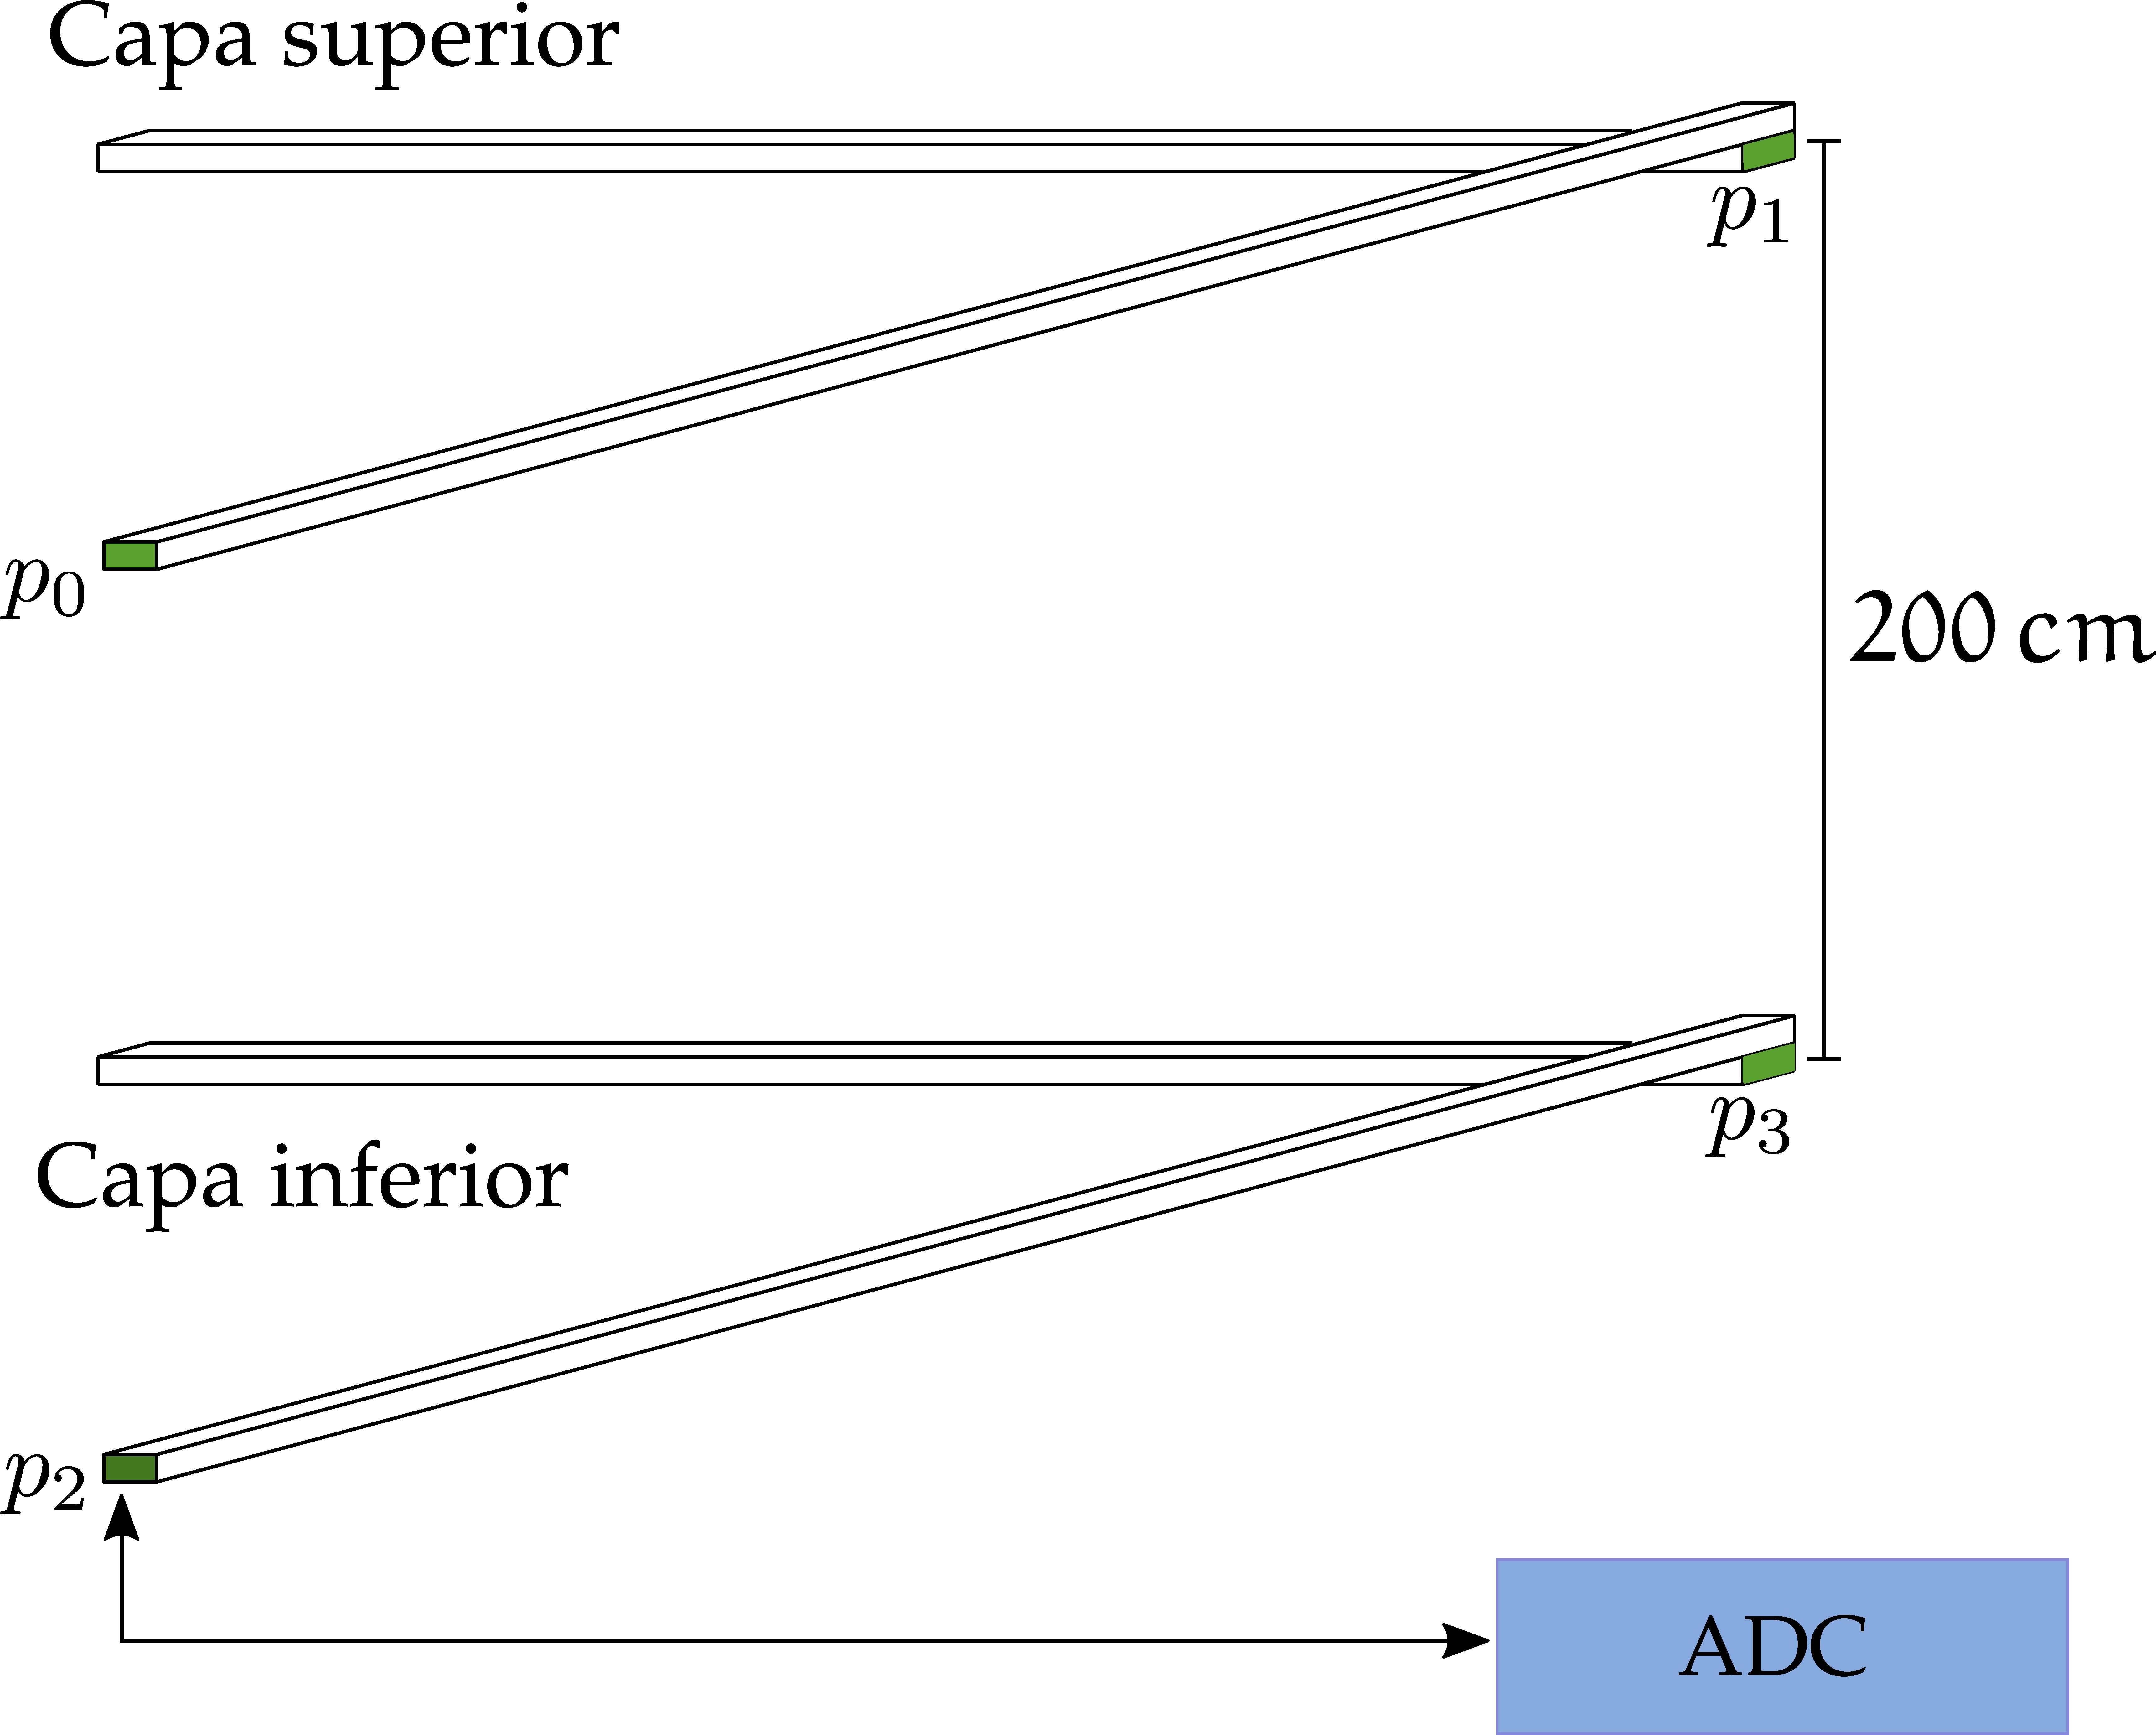
\includegraphics[width=\textwidth]{muons-experiment-0.pdf}
        \caption{Configuración del experimento en Sierra Negra. El sistema de coincidencias se forma por las tarjetas instaladas en las posiciones marcadas en verde.}
        \label{fig:muons-experiment-0}
\end{figure}

Con el fin de inyectar a la simulación un espectro de muones adecuado, utilicé como generador de eventos el modelo PARMA model 4.0 (\emph{PHITS-based Analytical Radiation Model in the Atmosphere}) \cite{sato15,sato16}, el cual es capaz de reproducir los datos de diferentes experimentos de astrofísica a diferentes profundidades atmosféricas, incluyendo la dependencia del ángulo cenital. Para calcular el espectro de $\mu^{\pm}$ en Sierra Negra, el modelo PARMA considera la profundidad atmosférica, rigidez umbral y el periodo de observación (para corregir efectos debidos a la actividad solar). El espectro de energía de los muones que llegan a la barra en la parte de inferior del detector calculado mediante PARMA se muestra en la figura \ref{fig:muons-spectrum}. Usando este \emph{setup} de simulación podemos obtener la energía depositada por las partículas en la barra, así como la cantidad de fotones que llegan al sensor y sus tiempos de arribo.

\begin{figure}
        \centering
        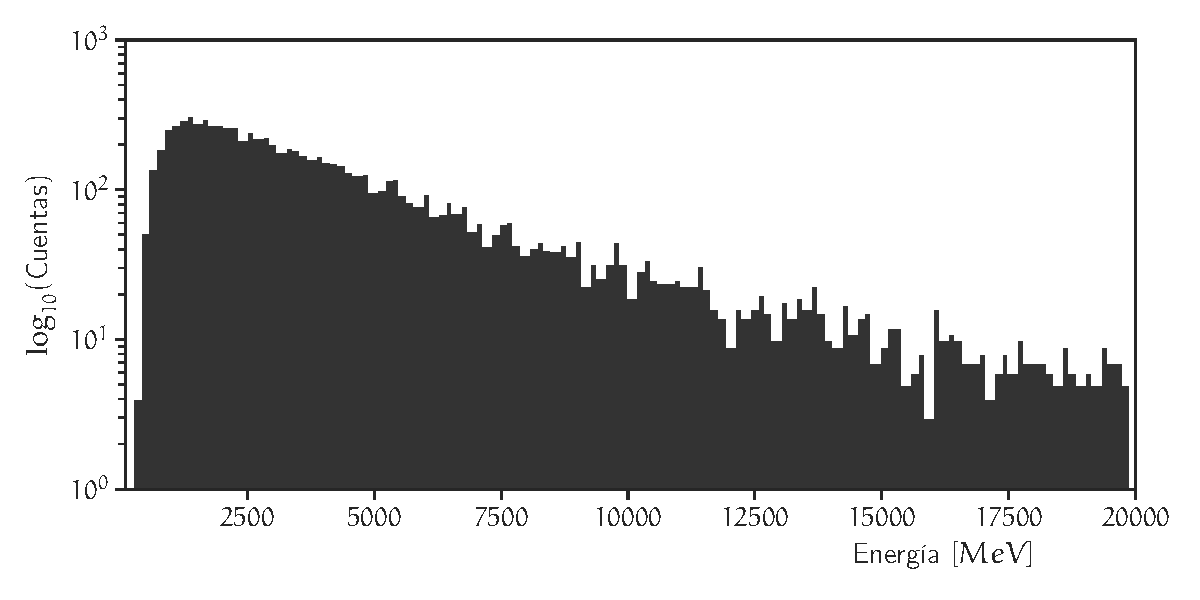
\includegraphics[width=\textwidth]{scibar-edep.pdf}
        \caption{Espectro de energía de $\mu^{\pm}$ utilizado en la simulación. El espectro es estimado a partir del modelo PARMA usando la localidad de Sierra Negra.}
        \label{fig:muons-spectrum}
\end{figure}

Un primer resultado que se observa de la figure \ref{fig:muons-spectrum} es que los muones que logran cruzar el SciCRT de forma vertical requieren al menos \SI{400}{\mega\electronvolt} de energía.

Puesto que la electrónica del SciCRT no permite procesar las señales de las barras de manera independiente, con el propósito de desarrollar el experimento, instalé en Sierra Negra cuatro amplificadores (marcados en verde en la figura \ref{fig:muons-experiment}) que desarrollé con la ayuda del Ing. Roberto Taylor, técnico en la estación de RC de Ciudad Universitaria.

La salida de los amplificadores genera la señal de \emph{$4$-fold}, la cual sirve como disparo para un digitalizador de pulsos, el cual toma la señal directa a la salida del fotomultiplicador (marcado como $p_{2}$). Con esta configuración obtenemos una tasa de eventos de \SI{275.3(30)}{eventos \per\hour}. El alto voltaje en los MAPMTs está fijo en \SI{-950}{\volt}, con un umbral en la electrónica de \SI{-70}{\milli\volt} (\SI{\sim 2}{pe}). Los pulsos registrados se muestrean a una frecuencia de \SI{4}{\giga muestras\per\second}.

La figura \ref{fig:muon-pulse} muestra en color azul oscuro una señal adquirida con el experimento, en comparación con señales producidas por la simulación (lineas de color). La simulación incluye todos los procesos descritos previamente: PARMA $+$ material absorbente $+$ barra de centelleo $+$ fibra WLS $+$ SPE del MAPMT.

\begin{figure}
        \centering
        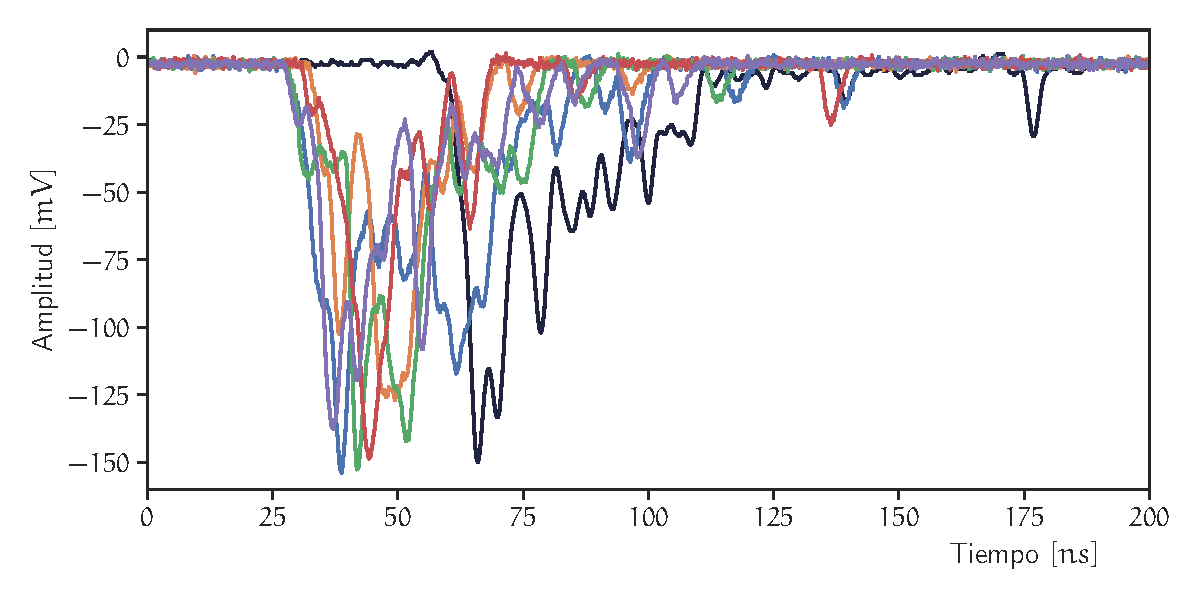
\includegraphics[width=\textwidth]{muon-pulse.pdf}
        \caption{Comparación entre señales generadas por la simulación MC (líneas de color) y el experimento realizado en Sierra Negra (línea oscura).}
        \label{fig:muon-pulse}
\end{figure}

De acuerdo con la simulación la tasa de eventos esperada para muones con energías mayores a \SI{400}{\mega\electronvolt}, atravesando verticalmente un área de \SI{6.25}{\cm\squared} es de \SI{264.6(15)}{eventos\per\hour}. Sin embargo, para poder comparar esta tasa con la tasa de experimento es necesario considerar la eficiencia de detección. Si analizamos el caso de una sola barra que registra más de \SI{2}{pe}, obtenemos que la eficiencia es cercana a $0.99$ y, dado que las barras producen señal de forma independiente, la eficiencia total es de $0.97$. Así, un mejor estimado de la tasa de eventos en la simulación es \SI{256.6(20)}{eventos\per\hour}.

A partir de aquí es posible observar que el experimento y la simulación difieren en la tasa de eventos en un \SI{7}{\percent}. En lo que sigue explicaré el origen de esta discrepancia, analizando las características en el tiempo y carga depositada por los muones registrados en el experimento.

En principio, la contaminación ocasionada por partículas de otras especies, capaces de cruzar el detector, es casi despreciable. Luego entonces, la mayor tasa en el experimento debe ser ocasionada por eventos multiples (dos o más partículas registradas en una ventana de \SI{200}{\ns}) o disparos accidentales.

El diagrama de tiempos de la generación de las señales en el experimento se muestra en la figura \ref{fig:muons-experiment-1}. La distancia entre el MAPMT y el punto donde el muon el cruza y genera la coincidencia es de \SI{295.0(25)}{\cm}. Los fotones emitidos desde este punto, dentro del centellador, requieren por lo menos de \SI{16}{\ns} para alcanzar el MAPMT (considerando que se propagan en línea recta). Este valor es ensanchado por la distribución angular de los fotones transmitidos por la reflexión total interna en la fibra y los fotones que se reflejan al final de la barra y el revestimiento. A partir de la simulación pude estimar que el tiempo mínimo que requieren los fotones para llegar al MAPMT es de \SI{23}{\ns} ($t_{A}$ en el diagrama). En el diagrama se observa que la señales adquiridas en los puntos $p_{0}$ y $p_{2}$ son afectadas por este retardo temporal. Por otro lado, los muones relativistas que cruzan el telescopio de forma vertical solo necesitan \SI{7}{\ns} (marcado como $t_{B}$) para alcanzar la parte inferior del detector. Siguiendo este razonamiento, las señales en $p_{1}$ ocurren casi inmediatamente después de la interacción de la partícula, mientras que los pulsos adquiridos en $p_{2}$ y $p_{3}$ están atrasados $t_{B}$ con respecto a las señales en el tope. Dado que los eventos en $p_{2}$ son los últimos en producirse, el instante en que ocurren determina el tiempo de generación de disparo.

\begin{figure}
        \centering
        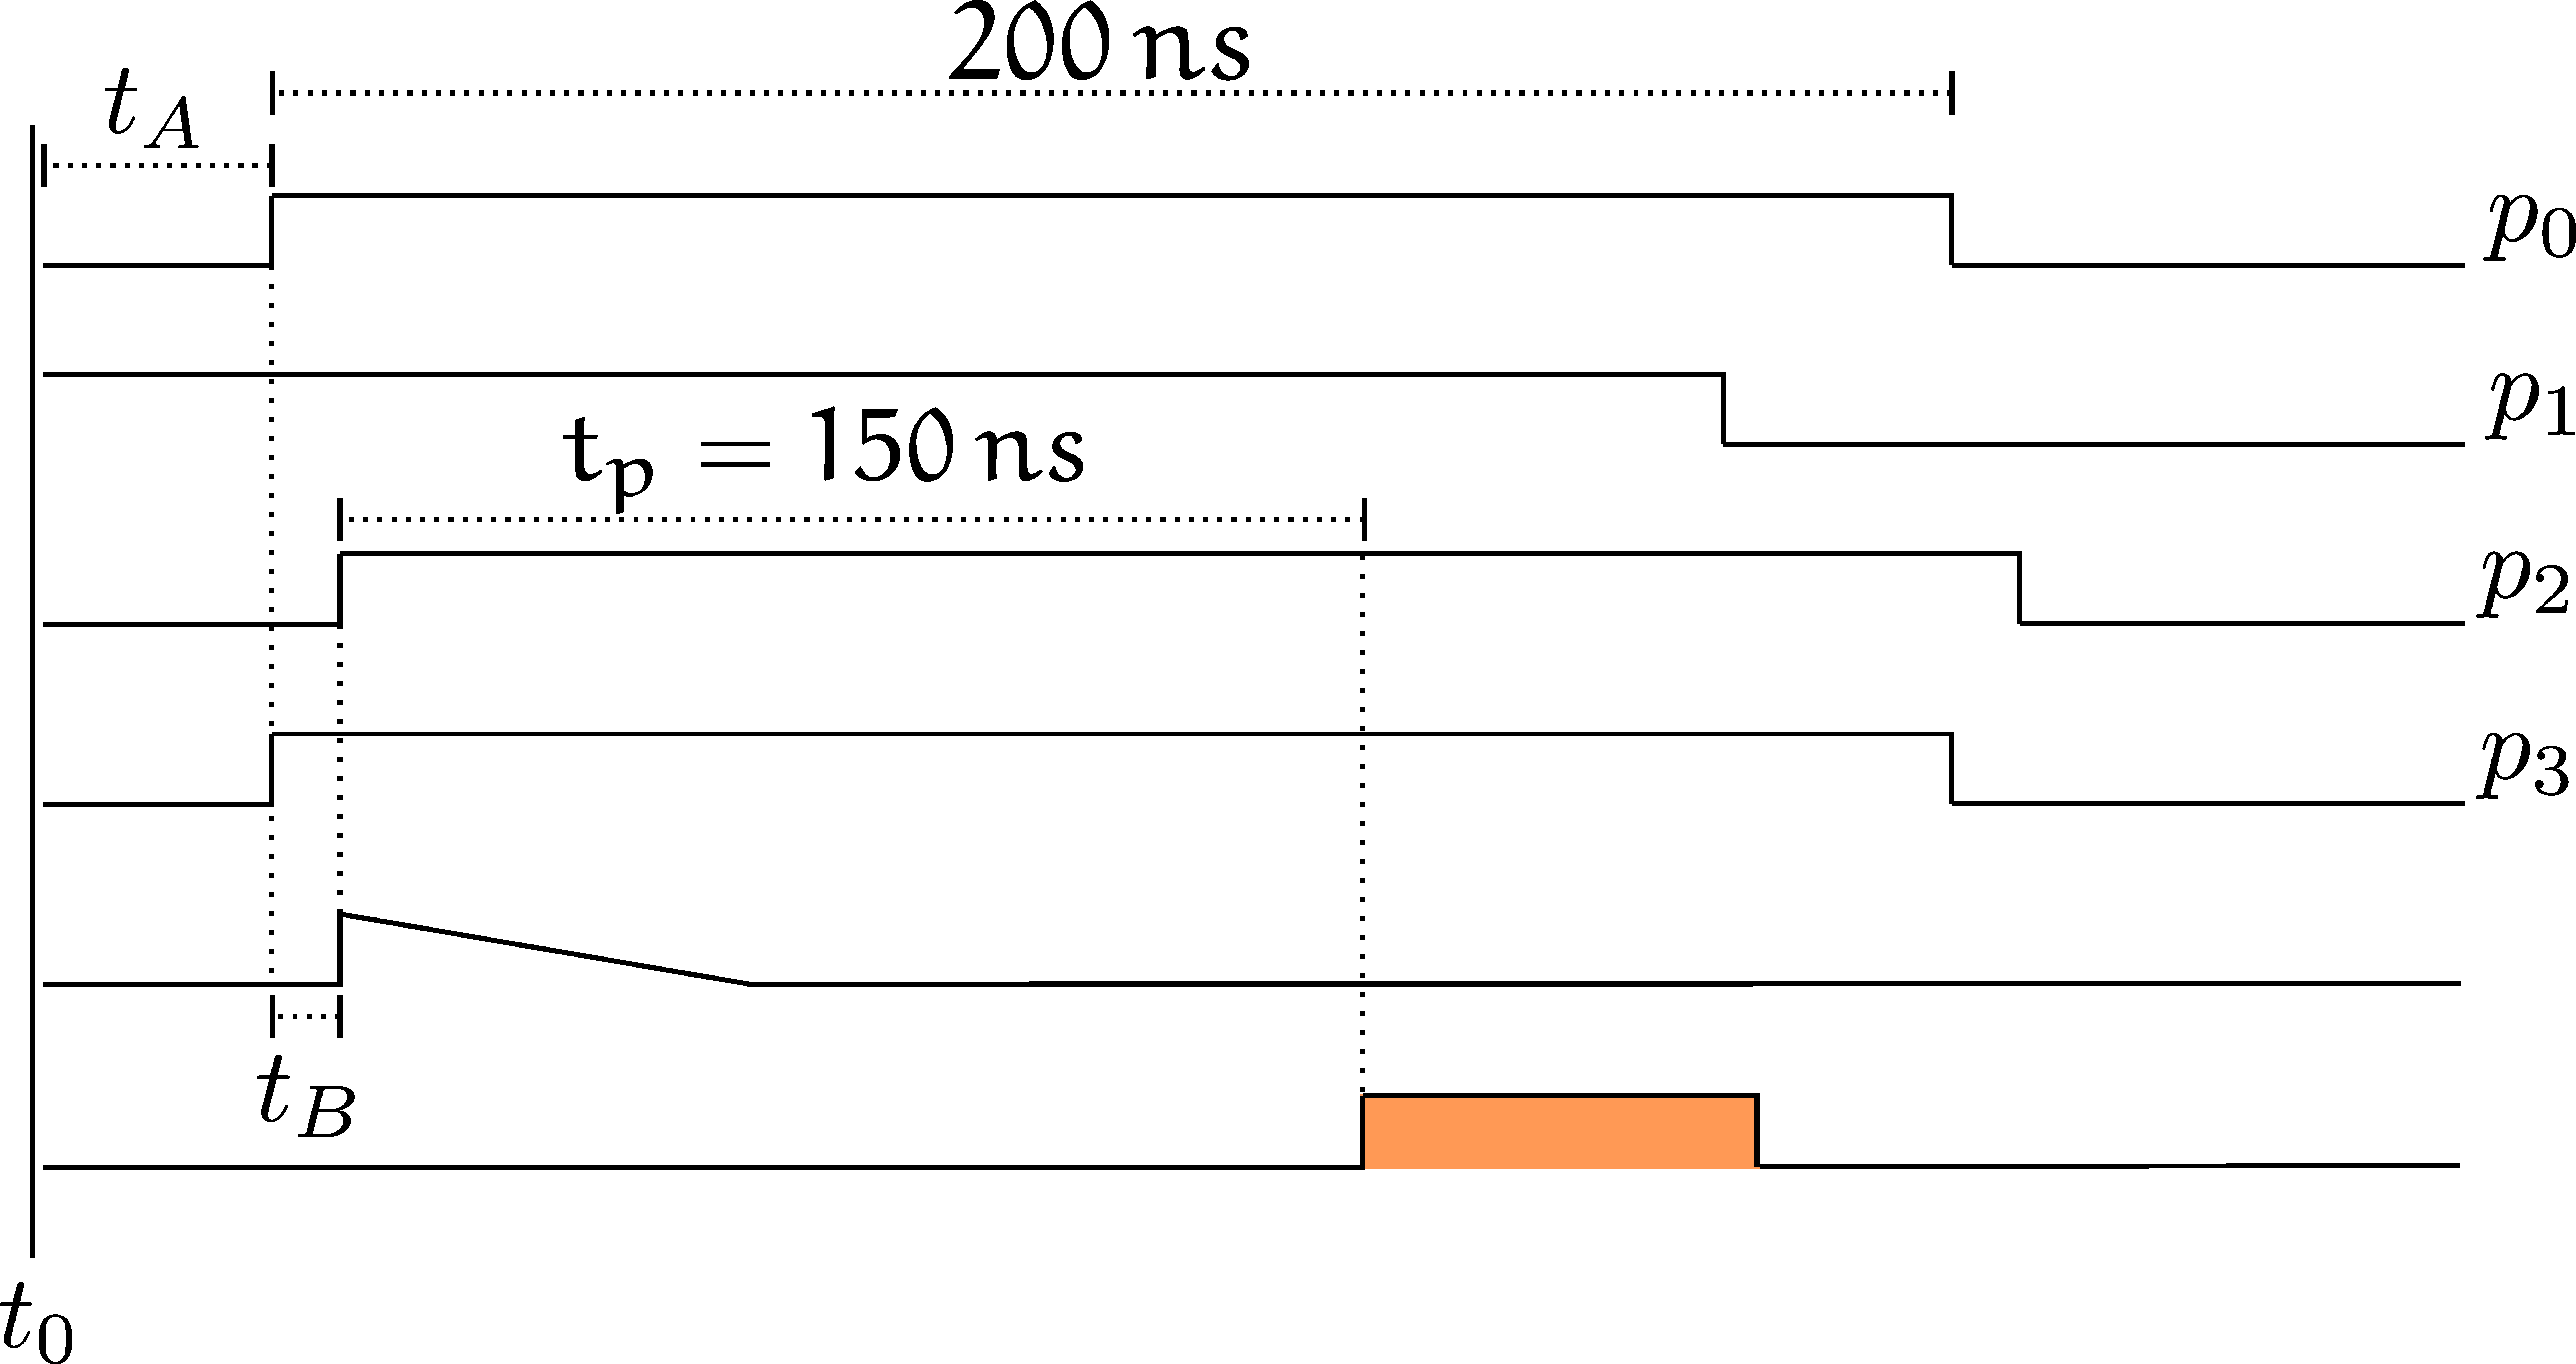
\includegraphics[width=\textwidth]{muons-experiment-1.pdf}
        \caption{Diagrama de tiempos de la generación de señales en el experimento con muones atmosféricos.}
        \label{fig:muons-experiment-1}
\end{figure}

A esto se suma un retardo introducido por los amplificadores, cables de interconexión y otros elementos en la cadena de procesamiento de la señal, lo cual en total suma un retardo $t_{p}=\SI{150}{\ns}$. Lo destacable de este análisis es que ambos efectos se pueden usar para corregir los datos, de manera que el efecto de $t_{p}$ se usa para compensar los datos experimentales, mientras que los datos de la simulación son compensados por el retardo de $t_{A}+t_{B}$.

Con esto podemos comparar las distribuciones de tiempo $t_{max}$ en las que los pulsos alcanzan su valor máximo. El resultado de este análisis se muestra en la figura \ref{fig:tmax}. La distribución en verde es el resultado de la simulación, mientras que el histograma negro corresponde a los datos obtenidos en el experimento. La diferencia entre ambas distribuciones es evidente y proviene principalmente de no linealidades en el cadena de procesamiento que no están completamente caracterizadas y no se pueden incluir en la simulación. El más importante de estos efectos es debido a las variaciones de temperatura en el lugar, lo cual afecta a los circuitos que generan la coincidencia y según el fabricante es del orden de \SI{\pm 10}{\ns}. La segunda fuente de error importante es el digitalizador de pulsos, el cual tiene una incertidumbre en su tiempo de propagación del orden de \SI{\pm 50}{\ns}. Dado que ambos factores se pueden asumir derivados de errores en la electrónica y en principio no afectan directamente el número de eventos registrados, podemos descartar su papel en las diferencias entre la simulación y el experimento.

\begin{figure}
        \centering
        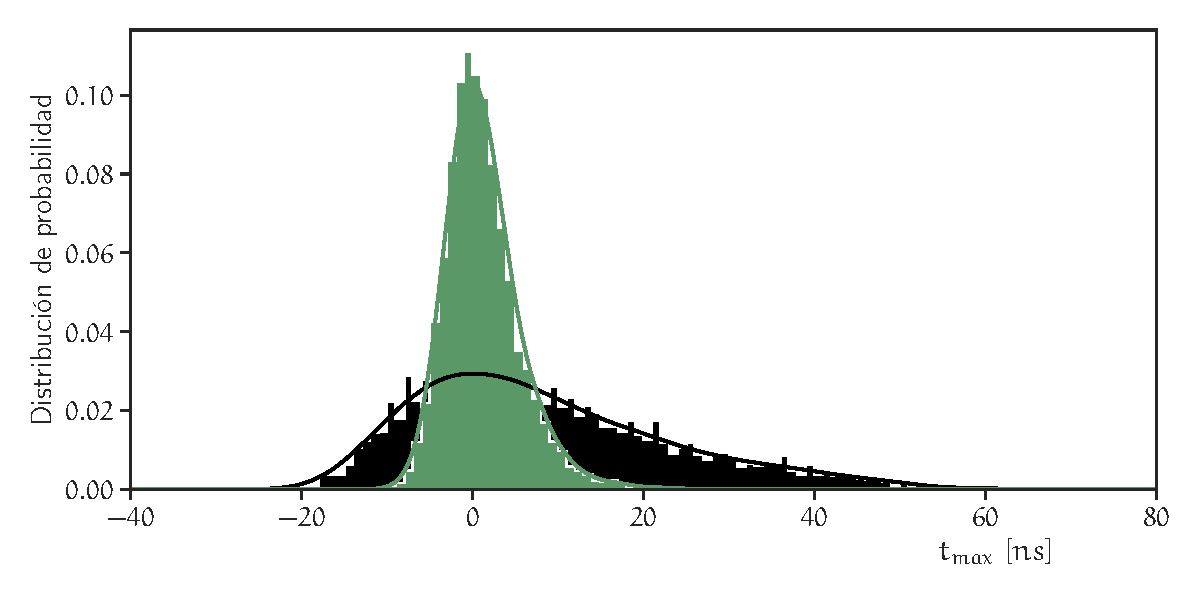
\includegraphics[width=\textwidth]{tmax_dist.pdf}
        \caption{Distribuciones de $t_{max}$ para el experimento y la simulación. La distribución en verde es el resultado de la simulación, mientras que la distribución en negra es proveniente del experimento.}
        \label{fig:tmax}
\end{figure}

Como se mencionó en la sección anterior, los fotones de centelleo y de la fibra son emitidos de forma aleatoria siguiendo un decaimiento exponencial. Resultado de este fenómeno, cada señal originada por la interacción de partículas en el plástico tiene la firma de un decaimento exponencial dominado por la constante de tiempo más lenta de los dos procesos. Para verificar esta característica, ajustamos una función exponencial negativa a la cola de todos los pulso, comenzando el instante de máxima amplitud. Los resultados se muestran en la figura \ref{fig:muons-tail}, en la cual las lineas punteadas representan los ajustes. Como se observa en la figura, el ajuste en los datos experimentales se limita a una ventana de \SI{50}{\ns} de duración. Esto es debido a que después de este instante la razón señal a ruido cae, lo que hace imposible seguir detectando el decaimiento. Los valores de constantes de tiempo obtenidas para la simulación y el experimento son: $\tau_{sim}=\SI{17.10(3)}{\ns}$, $\tau_{exp}=\SI{17.64(2)}{\ns}$, los cuales son cercanos a la constante de tiempo de la fibra WLS; la más lenta de ambas. Es de esperarse que este valor se degrade debido al volumen de la barra y el revestimiento \cite{gros18}.

\begin{figure}
        \centering
        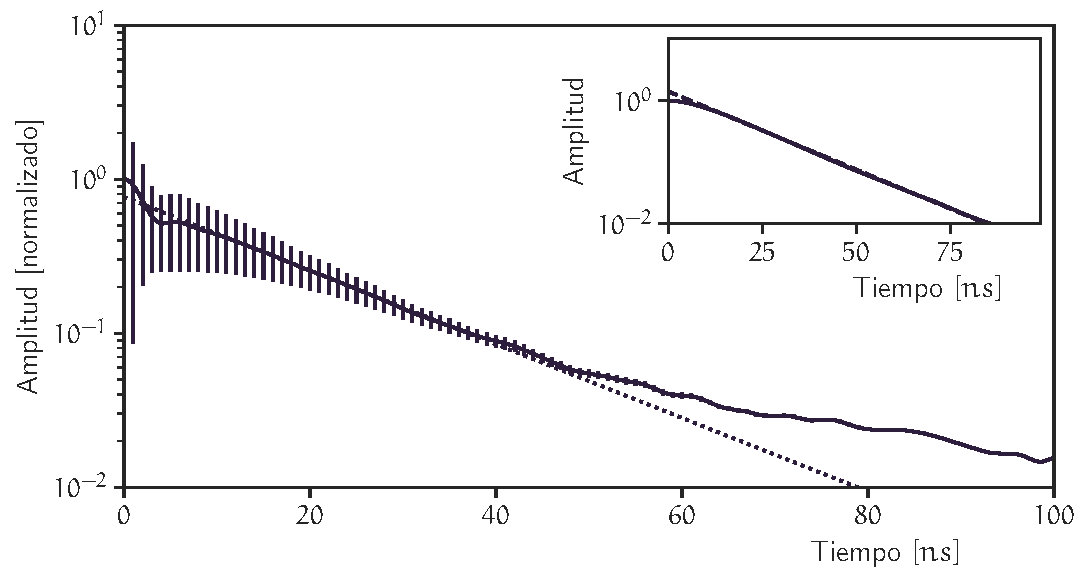
\includegraphics[width=\textwidth]{muons-tail-fit.pdf}
        \caption{Análisis del decaimiento exponencial de la fibra WLS. El panel en la esquina superior derecha muestra los resultados de la simulación. Los datos experimentales se muestran en la parte central de la figura.}
        \label{fig:muons-tail}
\end{figure}

A continuación analicé el ancho de las señales $t_{90}-t_{10}$, definido como el intervalo de tiempo que requiere el pulso para pasar del \num{10} al \SI{90}{\percent} de la carga total. La distribución color verde claro en la figura \ref{fig:t90-distribution} corresponde a los resultados de la simulación, mientras que la distribución negra proviene de los datos experimentales. Aunque ambas distribuciones son muy similares, se puede observar una diferencia de \SI{7}{\ns} entre los valores máximos de ambas. La razón de esto se encuentra en la degradación de los tiempos de subida y bajada de los pulsos debido al ancho de banda limitado de los elementos que componen la cadena de conexión. Si calculamos el tiempo de subida compuesto por estos elementos en serie obtenemos un valor de \SI{3.4}{\ns}, el cual además debe afectar a los pulsos de forma simétrica. De esta forma se explican de forma satisfactoria las diferencias entre experimento y simulación.

\begin{figure}
        \centering
        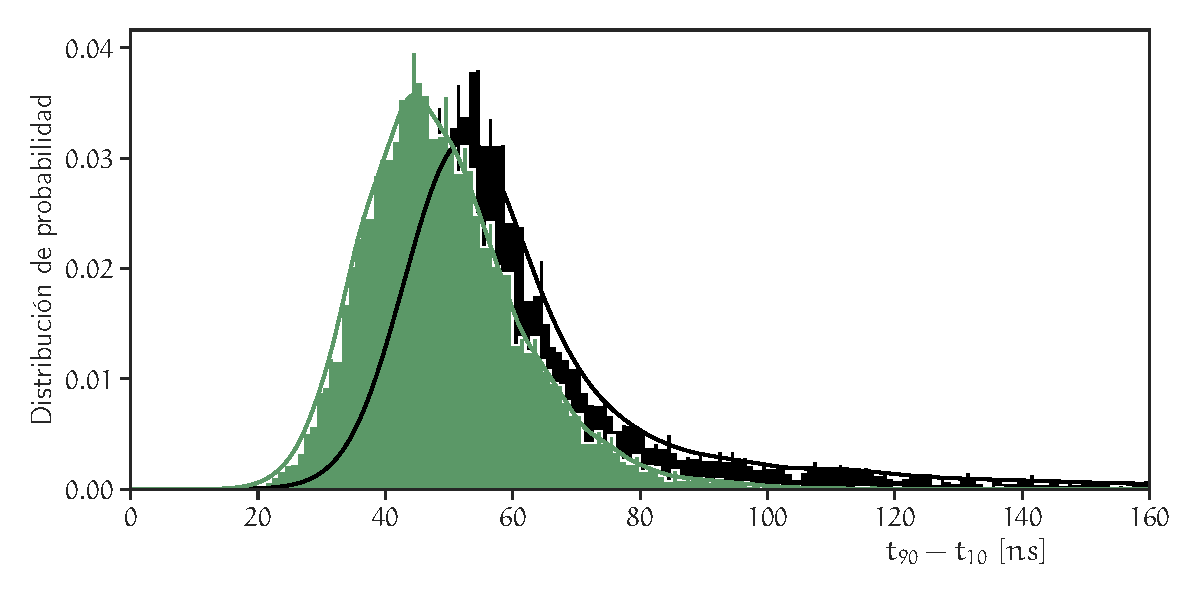
\includegraphics[width=\textwidth]{t90_dist.pdf}
        \caption{Distribuciones de ancho de pulso para datos experimentales y simulación. La distribución verde es el resultado de la simulación, mientras que la de color negro es el experimento.}
        \label{fig:t90-distribution}
\end{figure}

Otro rasgo distintivo de la distribución experimental es su cola más extendida, la cual se extiende más allá de los \SI{120}{\ns} y no puede ser corregida con los argumentos previos. Ya que el ancho del pulso es independiente de la energía depositada\footnote{Esto se debe a que la medida del ancho se hace sobre un pulso normalizado en amplitud.}, la cola de la distribución solo se puede atribuir a eventos de dos o más partículas en la ventana de tiempo o disparos accidentales. La figura \ref{fig:qtime-dist} muestra el histograma en dos dimensiones del número de fotoelectrones contra el ancho del pulso de los datos del experimento. La escala de colores representa el número de eventos en cada \emph{bin}. Como se observa en la figura los eventos con anchos mayores (mayores a \SI{100}{\ns}) se encuentran distribuidos en la parte de menor deposición de carga, lo cual supone no pueden ser originados por dos o más partículas. Por lo tanto suponemos la contaminación debe originarse de disparos accidentales de la electrónica. A partir de la simulación podemos estimar que la probabilidad de tener un pulso de ancho mayor a \SI{100}{\ns} es menor a \SI{0.5}{\percent}, así que establecemos esto como un umbral de corte para limpiar los datos experimentales. Después de la selección de eventos, la tasa de eventos registrada en el experimento es \SI{253.3(50)}{eventos\per\hour}.

\begin{figure}
        \centering
        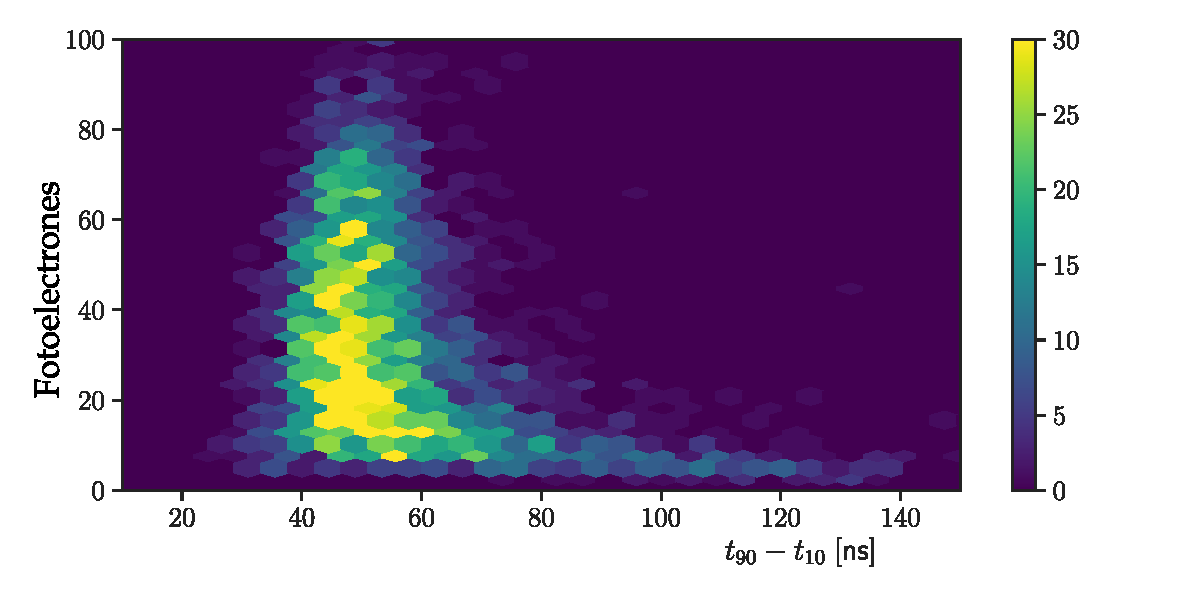
\includegraphics[width=\textwidth]{qtime-dist.pdf}
        \caption{Histograma en dos dimensiones mostrando la relación de $t_{90}-t_{10}$ y el número de fotoelectrones en la señal. La escala de colores representa el número de eventos en cada \emph{bin}.}
        \label{fig:qtime-dist}
\end{figure}

Finalmente, cerraré este capitulo comparando las distribuciones del número de fotoelectrones en el experimento y la simulación. La figura \ref{fig:photons-number} muestra los resultados. La línea verde corresponde a los datos del experimento, mientras que la linea negra representa la simulación. La diferencia entre ambas es de esperarse ya que la simulación no incluyen los efectos de la resolución finita del detector y otras no linealidades. El efecto de la resolución finita puede agregarse a la simulación sumando la contribución de una variable aleatoria Gaussiana. Este proceso se puede representar mediante la ecuación \ref{equ:nphe}, la cual describe la convolución de la distribución de fotoelectrones con la función de resolución $p(N_{phe})$:

\begin{equation}
\label{equ:nphe}
s(N_{phe})=\frac{1}{k_{sat}}\int_{0}^{N_{max}} s_{sim}(N_{sim})p(N_{phe}-N_{sim})\;\mathrm{d}N_{sim}
\end{equation}

de donde $s$ representa la distribución experimental y $s_{sim}$ la obtenida mediante simulación. El efecto de la resolución del detector en la distribución experimental es evidente si comparamos los valores máximos de ambas distribuciones, centrados alrededor de \SI{10}{pe}. De esta forma el ensanchamiento en la distribución del experimento se puede explicar considerando las fluctuaciones aleatorias en la respuesta. Por otra parte, el cambio de variable de $N_{phe}$ (número observable de fotoelectrones) y $N_{sim}$ indica la distorsión ocasionada por una respuesta no lineal. En este sentido introducimos la función de saturación $k_{sat}$, la cual modela la posible saturación del MAPMT al trabajar a voltajes cercanos a su límite de operación. Para este análisis use un polinomio de segundo orden como función de saturación para ajustar la simulación a los datos experimentales.

\begin{figure}
        \centering
        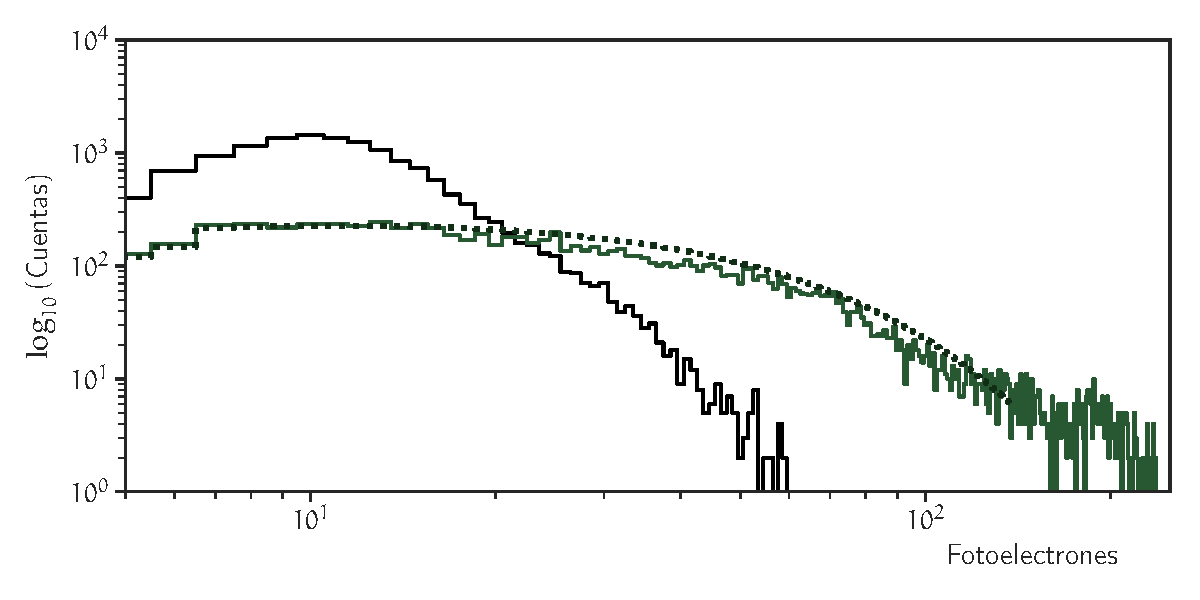
\includegraphics[width=\textwidth]{photons-number.pdf}
        \caption{Distribución de número de fotoelectrones detectados en el experimento y la simulación MC. Los resultados de la simulación se convolucionan con una función de resolución para ajustar con los datos experimentales (ver texto).}
        \label{fig:photons-number}
\end{figure}

La línea punteada en la figura \ref{fig:photons-number} muestra los resultados de la simulación al incorporar los efectos mencionados previamente. Tras la corrección los datos experimentales y la simulación concuerdan en el rango de \num{5} a \SI{150}{pe}. Para valores de carga mayores los motivos de la desviación no son evidentes, lo cual podría suponer un cambio en la función de saturación o alguna otra no linealidad. De cualquier manera, con este análisis concluimos que la deposición de energía de $\mu^{\pm}$ tiene un valor máximo de \SI{250}{pe}. Es importante enfatizar que, dado que el SciCRT opera de forma regular con una ganancia menor. los efectos de saturación y resolución aquí expresados no deben afectar significativamente el desempeño del telescopio.
